%%%%%%%%%%%%%%%%%%%%%%%%%%%%%%%%%%%%%%%%%
% Short Sectioned Assignment
% LaTeX Template
% Version 1.0 (5/5/12)
%
% This template has been downloaded from:
% http://www.LaTeXTemplates.com
%
% Original author:
% Frits Wenneker (http://www.howtotex.com)
%
% License:
% CC BY-NC-SA 3.0 (http://creativecommons.org/licenses/by-nc-sa/3.0/)
%
%%%%%%%%%%%%%%%%%%%%%%%%%%%%%%%%%%%%%%%%

%----------------------------------------------------------------------------------------
%	PACKAGES AND OTHER DOCUMENT CONFIGURATIONS
%----------------------------------------------------------------------------------------

\documentclass[paper=a4, fontsize=12pt, xcolor=dvipsnames]{scrartcl} % A4 paper and 11pt font size

\usepackage[T1]{fontenc} % Use 8-bit encoding that has 256 glyphs
\usepackage{fourier} % Use the Adobe Utopia font for the document - comment this line to return to the LaTeX default
\usepackage{amsmath,amsfonts,amsthm} % Math packages
\usepackage{natbib}
\usepackage{pgfplots}
\usepackage{wrapfig}
\usepackage{sidecap}
\usepackage{color, colortbl}  
%\usepackage[pass,showframe]{geometry} % just to show the margins
%\usepackage{booktabs}
%\usepackage{minted}

% Bibliographie auf deutsch
%\usepackage{harvard}
%\renewcommand{\harvardand}{und} 
\usepackage{caption}
\usepackage{xcolor}
\usepackage[utf8]{inputenc} 
%\usepackage[ngerman]{babel}

\usepackage{latexsym}
\usepackage{textcomp}
\usepackage[T1]{fontenc}
\usepackage{bm}% bold math
\usepackage{hyperref}
\usepackage{graphicx}
\usepackage{caption}
\usepackage{subcaption}
\usepackage{verbatim}
\usepackage{epsfig}
\usepackage{framed,color}
\usepackage{placeins}   % FloatBarrier
\usepackage[usenames,dvipsnames]{pstricks}
\usepackage{epsfig}
\usepackage{tikz}
\usepackage{lipsum} % Used for inserting dummy 'Lorem ipsum' text into the template
\usepackage{sectsty} % Allows customizing section commands
\usepackage{hyperref}
\allsectionsfont{\centering \normalfont\scshape} % Make all sections centered, the default font and small caps

\usepackage{fancyhdr} % Custom headers and footers
\pagestyle{fancy} % Makes all pages in the document conform to the custom headers and footers
\renewcommand{\headrulewidth}{0.0pt} % Remove header underlines
\renewcommand{\footrulewidth}{0pt} % Remove footer underlines

\setlength{\headheight}{13.6pt} % Customize the height of the header
\usepackage{eso-pic}
\numberwithin{equation}{section} % Number equations within sections (i.e. 1.1, 1.2, 2.1, 2.2 instead of 1, 2, 3, 4)
\numberwithin{figure}{section} % Number figures within sections (i.e. 1.1, 1.2, 2.1, 2.2 instead of 1, 2, 3, 4)
\numberwithin{table}{section} % Number tables within sections (i.e. 1.1, 1.2, 2.1, 2.2 instead of 1, 2, 3, 4)

\setlength\parindent{0pt} % Removes all indentation from paragraphs - comment this line for an assignment with lots of text
\setcapindent{1cm} 

%----------------------------------------------------------------------------------------
%	TITLE SECTION
%----------------------------------------------------------------------------------------

\title{ 
\normalfont \normalsize 
\textsc{Albert-Ludwigs-University Freiburg} \\ [25pt] % Your university, school and/or department name(s)
\horrule{0.5pt} \\[0.4cm] % Thin top horizontal rule
\huge \textsc{Faraday and Pockels effect} \\ % The assignment title
\horrule{2pt} \\[0.5cm] % Thick bottom horizontal rule
}


\author{Friedrich Schüßler and Volker Karle} % Your name

\date{\normalsize\today} % Today's date or a custom date


%--------------------------------------------------------------------------------------------
% New Commands
%--------------------------------------------------------------------------------------------
\newcommand{\horrule}[1]{\rule{\linewidth}{#1}} % Create horizontal rule command with 1 argument of height


\begin{document}

\blendcolors*{!83}\color{black}
\maketitle
\begin{center}
 
\includegraphics[width=0.6\linewidth]{figures/unifreiburg}
\end{center}
\thispagestyle{empty}
\newpage
    {\pagestyle{plain}
    \thispagestyle{empty}
    \tableofcontents
    \thispagestyle{empty}
    \cleardoublepage}
\newpage


%----------------------------------------------------------------------------------------
%	PROBLEM 1
%----------------------------------------------------------------------------------------
% This file contains all the new commands defined 
% in order to facilitate the writing of the latex code. 
% It has to be loaded into the main .tex file at the beginning!

\newcommand{\nn}{\nonumber \\}
\newcommand{\beq}{\begin{equation}}
\newcommand{\eeq}{\end{equation}}
\newcommand{\beqn}{\begin{equation*}}   % equation without numbering
\newcommand{\eeqn}{\end{equation*}}
\newcommand{\bea}{\begin{eqnarray}}
\newcommand{\eea}{\end{eqnarray}}
\newcommand{\bean}{\begin{eqnarray*}}
\newcommand{\eean}{\end{eqnarray*}}
\newcommand{\bit}{\begin{itemize}}
\newcommand{\eit}{\end{itemize}}

\newcommand{\E}{\mathbf{E}}
\newcommand{\D}{\mathbf{D}}
\newcommand{\B}{\mathbf{B}}




\setcounter{page}{1}
\subsection{Overview}
In the following experiment, we will analyse the spectral band of absorbtion of the iodine 2 molecule 
with spectroscopal methods. For the given conditions, the expected observation stems almost 
entirely from one electronic transition, the 
\begin{equation}
    B ^3\Pi_{\sigma \, \mathrm{u}}^{+} \quad <- \quad X ^1\Sigma_{\sigma \, \mathrm{u}}^{+}
\end{equation}
transition. Since iodine is a relativly heavy di-atomic molecule, it has vibrational modes that 
split up the total energy of the molecule considerably and are visible in the spectrum with the 
resolution of the given spectrometer. The energy is further changed by rotational modes of the 
atoms, which however don't show up as separate lines but rather widen the observed bands, as the 
resolution is not high enough. 
The observed data is then used to calculated characteristical constants for the molecule, such as 
the dissipation energy $D_e$ and the mean radius $r_c$. 

\subsection{Historic review}
The structure of molecular iodine ($I_2$) has been studied various times in physical chemistry 
during the last century. One of the first thorough measurements of the spectral bands was done in 
1923 by the German physicist Reinhard Meck \cite{mecke1923bandenspektrum}. The vibrational states 
were correctly numbered for the first time by Loomis \cite{loomis1927correlation}, who analysed 
the fluorecence spectrum earlier measured by Wood \cite{wood1911} for $v = 26$.



\clearpage

% Pockels
\section{Theory behind the Pockels effect}

\subsection{Light propagating in matter}
\paragraph{The basis of discussing} 
electro-optical effects are 
Maxwell's equations in matter~\cite{boyd2003nonlinear}:
\begin{subequations} 
\begin{align}
\nabla \cdot \D &= \rho_\text{f} 
\label{eq:max1} \\ 
\nabla \cdot \B &= 0
\label{eq:max2} \\ 
\nabla \times \E &= -\frac{\partial \B} {\partial t}
\label{eq:max3} \\ 
    \nabla \times \mathbf{H} &= \mathbf{J}_\text{f} + 
        \frac{\partial \D} {\partial t}, 
\label{eq:max4}
\end{align}
\label{eq:maxwell}
\end{subequations}
where 
\begin{itemize}
    \item $\D$ is the electric displacement field, related to the eletric field $\E$ 
    by the constitutive equation 
    \begin{equation}
        \D = \eps_0 \Eps \E 
    \label{eq:const1}
    \end{equation}
    where $\Eps$ is the dielectric tensor and $\eps_0$ is the permittivity of free 
    space; 
    \item $\mathbf{H}$ is the magnetizing field, with the constitutive equation 
    \begin{equation}
        \mathbf{H} = \mu^{-1} \, ;
    \label{eq:const2}
    \end{equation}
    \item $\mathbf{J}_\text{f}$ is the free current density, and
    \item $\mathbf{\rho}_\text{f}$ is the free charge density.
\end{itemize}
Equations \eqref{eq:const1} and \eqref{eq:const2} are valid for materials without 
coupling between magnetic and eletric fields, which is the case in our 
crystal. We are, however, facing an anistropic material, so that 
$\Eps$ is a tensor, while we assume the permeability $\mu$ of the material 
to be just the vacuum permeability $\mu_0$, such that
$\B = \mu \mathbf{H} = \mu_0 \mathbf{H}$. 
If we assume $\mathbf{\rho}_\text{f} = 0$, $\mathbf{J}_\text{f} = 0$ 
(no free charge and currents), we obtain the homogenious 
Maxwell equations. By applying the curl operator $\nabla \times$ 
to \eqref{eq:max3}, we get the wave equation 
\begin{equation}
    - \Delta \E + \frac{\eps}{\eps_0 c^2} \frac{\partial^2 \E}{\partial t^2}  = 0
    \label{eq:wave_eq}
\end{equation}
which possesses plane waves as solutions, 
described by
\begin{subequations}
\begin{align}
    \E &= \En \exp \left[i(\mathbf{k \cdot r}-\omega t)\right] \\
    \mathbf{H} &= \mathbf{H_0} \exp \left[i(\mathbf{k \cdot r}-\omega t)\right], 
\end{align}
\end{subequations}

Inserting into \eqref{eq:max3} and \eqref{eq:max4} yields:
\begin{subequations}
\begin{align}
    \mu_0 \omega \mathbf{H} &= \K \times \E 
    \label{eq:plan_H} \\
    \omega \D &= - \K \times \mathbf{H}.
    \label{eq:plan_D} 
\end{align}
\end{subequations}
We observe, that $\K, \D$, and $\Ha$ are mutually perpendicular. 
Looking at the energy flux
\begin{equation}
    \mathbf{S} = \E \times \Ha, 
\end{equation}
we further see, that the directions of $\mathbf{S}$ and $\K$ do not 
coincide if $\E \nparallel \Eps \E$. 

\paragraph{As a consequence}, 
plane waves can be polarized in any direction 
perpendicular to $\K$. Linear polarized waves conserve the 
direction of polarization in time and space. They are formed 
the superposing two waves with the same frequency and a 
relative phase $\Delta \phi = n \pi$, where $n \in \mathbb{Z}$. 
Any linearly polarized wave can be split up into two orthogonal 
components of equal amplitude, each forming an angle of $45^\circ$ 
with the original polarization.
A linear combination of two aves of the same frequency $\omega$, 
wavevector $\K$ but orthogonal polarization and a fixed phase 
difference $\Delta \phi \neq 0$ is generally polarized elliptically.
For the special case of equal amplitudes and $\Delta \phi = \pi /2$,
the polarization is circular. 

\paragraph{In order to asses} 
the differences in phase induces by the Pockels effect, we need to 
relate refraction to the phase. To do so, we look at two plane waves  
\begin{align}
\E_1(\mathbf{r}, t) = (\E_1)_0 \exp\left\{i(\K_1 \cdot \mathbf{r} - \omega t) \right\} \\ 
\E_2(\mathbf{r}, t) = (\E_2)_0 \exp\left\{i(\K_2 \cdot \mathbf{r} - \omega t) \right\} \\ 
\end{align}
with the same frequency $\omega$,
we can define $\Delta \phi$ at 
one time $t$ and position $\mathbf{r}$ by 
\begin{equation}
    \Delta \phi := \left(\K_2 - \K_1 \right) \cdot \mathbf{r}\, .
\end{equation}
By the definition of $\N$ \eqref{eq:def_n} and the identity 
\begin{equation}
    \omega = \frac{2 \pi c}{\lambda} \, ,
\end{equation}
we can write 
\begin{equation}
    \Delta \phi = \frac{2 \pi}{\lambda} 
    \left(\N_2 - \N_1 \right) \cdot \mathbf{r} \, .
\end{equation}
If we further assume $\N$ to be parallel to $\mathbf{r}$, 
and measure $\Delta \phi$ after the two waves passed 
through a crystal of lenght $l$, then we get
\begin{equation}
    \Delta \phi_l = \frac{2 \pi}{\lambda} 
    \left(n_2 - n_1 \right) l \, .
    \label{eq:dphi}
\end{equation}


\subsection{Birefringence}
\paragraph{If the refraction index}
 $n$ of a material depends on the linear polarization of light, 
then a beam of light propagating in the material will be split up into 
two beams with perpendicular polarization and different propagation speed 
\begin{equation}
   v_i = \frac{c}{n_i}, 
\end{equation}
In order to explain this phenomenon, it is helpful to examine the 
structure of the material and connected quantities, as well as 
to retrieve the way light propagates by looking at the solutions 
of Maxwell's equations in matter \eqref{eq:maxwell}.
If we define the 
refractive index $\mathbf{n}$ by 
\begin{equation}
    \K = \frac{\omega}{c} \N \, ,
    \label{eq:def_n}
\end{equation}
we can rewrite equations \eqref{eq:plan_H} and \eqref{eq:plan_D} as 
\begin{subequations}
\begin{align}
    \mathbf{H} &= \frac{1}{\mu_0 c} \N \times \E 
    \label{eq:plan_Hb} \\
    \D &= - \frac{1}{c} \N \times \mathbf{H}
    \label{eq:plan_Db} \, .
\end{align}
\end{subequations}
Inserting the latter one into the first and using 
the identity $c^2 = \frac{1}{\mu_0 \eps_0}$, we get 
\begin{equation}
    \begin{split}
    \D  &= \frac{1}{\mu_0 c^2} \N \times \left(\E \times \N\right) \\
        &= \eps_0 \left(n^2 \E - \left(\N \cdot \E\right) \N \right)
    \label{eq:D(E)}
    \end{split}
\end{equation}
With the constitutive equation \eqref{eq:const1}, we obtain three 
equations linear in the components $E_k$:
\begin{equation}
    \left(n^2 \delta_{ik} - n_i n_k - \epsilon_{ik}\right) E_k = 0
\end{equation}
This equation is solve if its determinant vanishes:
\begin{equation}
    \mathrm{det}\,\left|n^2 \delta_{ik} - n_i n_k - \epsilon_{ik}\right| = 0
\end{equation}
By applying the principle axis theorem~\cite{strang2003introduction}, 
we can write $\Eps$ as the diagonal matrix with elements $\eps_x, \eps_y, \eps_z$. 
This yields \emph{Fresnel's equation}:
\begin{align}
    n^2 \left(\eps_x n_x^2 + \eps_y n_y^2 + \eps_z n_z^2 \right) 
    - \left[
        n_x^2 \eps_x \left(\eps_y + \eps_z\right) + 
        n_y^2 \eps_y \left(\eps_z + \eps_x\right) + 
        n_z^2 \eps_z \left(\eps_x + \eps_y\right) 
    \right] + \nonumber \\
    + \quad \eps_x \eps_y \eps_z = 0
    \label{eq:fresnel}
\end{align}
Being of second order in $n_i^2$, $i \in \{x, y, z\}$, there are up to two linearly 
independent solutions, corresponding to two possible directions of polarization. 


\paragraph{The case of a uniaxial crystal} 
is especially easy to solve. 
If we take the $z$-axis to be that of rotational symmetry, 
we can rename the components of 
$\Eps$ with 
\begin{align}
\eps_x &= \eps_y = \eps_\perp 
\label{eq:eps_perp}\\
\eps_z &= \eps_\parallel \, .
\label{eq:eps_parallel}
\end{align}
The $z$-axis is also called the \emph{optical axis}.
Fresnel's equation \eqref{eq:fresnel} can then be factored into
\begin{equation}
    \left(n^2 - \eps_\perp\right) 
    \left[\eps_\parallel n_z^2 + 
        \eps_\perp \left(n_x^2 + n_y^2\right) -
        \eps_\perp \eps_\parallel 
    \right] = 0 \, .
\end{equation}
In other words, we have two quadratic equations
\begin{align}
    n^2 &= \eps_\perp
    \label{eq:sphere} \\
    n_z^2 \eps_\perp + \left(n_x^2 + n_y^2\right) \eps_\parallel &= 1
    \label{eq:ellipsoid}
\end{align}
Equation \eqref{eq:sphere} gives a sphere for the wave-vector surface. To the 
corresponding types of waves, the crystal behaves like an isotropic body, being 
characterized by the refractive index $n = \sqrt{\eps_\perp}$. These waves are 
called \emph{ordinary waves}. The second type, accordingly named 
\emph{extraordinary waves}, is confined by the ellipsoid \eqref{eq:ellipsoid}. 
It's magnitude depends on 
the angle $\theta$ to the optical axis by 
\begin{equation}
    \frac{1}{n^2} =  \frac{\sin^2 \theta}{\eps_\parallel} - 
        \frac{\cos^2 \theta}{\eps_\perp} \, .
    \label{eq:theta}
\end{equation}

\paragraph{In order to relate} 
these two surfaces to two directions of polarization and 
determine the direction of a ray, we introduced the \emph{ray vector} $\mathbf{s}$, 
which is defined by the direction of the group velocity
\begin{equation}
    \frac{\partial \omega}{\partial \K}
\end{equation}
and the magnitude fullfilling 
\begin{equation}
    \mathbf{s} \cdot \N = 1\,.
\end{equation}
The ray vector defines the \emph{ray surface} by the condition 
$\phi = \mathrm{const.}$ 
for all $\mathbf{s}$ on that surface, where $\phi$ is the phase of the wave. 

We can show that $\mathbf{s} \parallel \mathbf{S}$: Differentiating 
equations \eqref{eq:plan_Hb} and \eqref{eq:plan_Db}, we get 
\begin{subequations}
\begin{align}
    c \delta \D &= \delta \Ha \times \N + \Ha \times \delta \N \\
    \mu_0 c \delta \Ha &= \N \times \delta \E + \delta \N \times \E \, ,
\end{align}
\end{subequations}
which by multiplying with $\E$ and $\Ha$, respectively, and applying 
basic properties of vector and scalar products, yield
\begin{subequations}
\begin{align}
    \begin{split}
    c \E \cdot \delta \D 
    &= \E \cdot \left(\delta \Ha \times \N \right) + 
        \E \cdot \left(\Ha \times \delta \N \right) \\
    &= \delta \Ha \cdot \left(\N \times \E \right) + 
        \delta \N \cdot \left(\E \times \Ha \right)  \\
    &= \mu_0 c \Ha \cdot \delta \Ha + 
        \delta \N \cdot \left(\E \times \Ha \right)
    \end{split} \\
    \mu_0 c \Ha \cdot \delta \Ha &= c \D \cdot \delta \E + 
        \delta \N \cdot \left(\E \times \Ha \right) \, ,
\end{align}
\end{subequations}
using again \eqref{eq:plan_Hb} and \eqref{eq:plan_Db}. It follows directly, that 
\begin{equation}
    \delta \N \cdot \left( \E \times \Ha \right) = \delta \N \cdot \mathbf{S} = 0 \, .
\end{equation}
To show, that $\se$ and $\mathbf{S}$ have the same direction, we need to show, 
that $\se$ is orthogonal on the surface of the wave vector surface, or, since 
the infinitesimal displacement $\delta \N$ lies 
on that surface, that $\se \cdot \delta \N = 0$. 
The wave vector surface given by \eqref{eq:fresnel} can be described by 
$f(\omega, \K) = 0$, which implies 
\begin{equation}
    \frac{\partial \omega}{\partial \K} = 
    - \frac{\partial f / \partial \K}{\partial f / \partial \omega}
\end{equation}
for the group velocity and thus 
\begin{equation}
    \se \parallel \frac{\partial f }{\partial \K} \parallel \frac{\partial f}{\partial \N}
    \label{eq:s_dir}
\end{equation}
since the gradient along $\K$ is taken for constant $\omega$. $\partial f / \partial \N$, however, 
is normal to the surface $f = 0$, so we can conclude, that
\begin{align}
    \se \cdot \delta \N &= 0 \\
    \Rightarrow \qquad \se &\parallel \mathbf{S} \, .
\end{align}
If follows, that 
\begin{equation}
    \se \cdot \Ha = 0 \qquad \se \cdot \E = 0 \, .
    \label{eq:coplanar}
\end{equation}
For uniaxial crystals, we can specify the ray surface in a form similar to 
\eqref{eq:ellipsoid} by doing analoge calculations with the folloing substitutions:
\begin{equation}
    \E \leftrightarrow c \D \, ; 
    \qquad \N \leftrightarrow \mu_0 c \se \, ; 
    \qquad \eps_{ik} \leftrightarrow {\eps^{-1}}_{ik} \, .
\end{equation}
The result is 
\begin{align}
    s^2 &= \eps_\perp
    \label{eq:s_sphere} \\
    {s_z}^2 \eps_\perp + \left( {s_x}^2 + 
        {s_y}^2\right) \eps_\parallel &= 1 \, .
    \label{eq:s_ellipsoid}
\end{align}
Since $\eps_x = \eps_y$, $\N$ and $\se$ must be coplanar with the optical axes. This 
common plane is called \emph{principal axis} for a given $\N$. Let this plane be 
defined by the $xz$-plane. We can get the direction 
of $\se$ from the relation \eqref{eq:s_dir}, namely by taking the derivatives of 
\eqref{eq:ellipsoid} with respect to $n_x$ and $n_z$:
\begin{equation}
    \frac{s_x}{s_z} = \frac{\eps_\perp n_x}{\eps_\parallel n_z} \, .
\end{equation}
The angle $\theta'$ between optical axis and ray vector is given in terms of 
$\theta$, as defined in equation \eqref{eq:theta}:
\begin{equation}
    \tan \theta' = \frac{\eps_\perp}{\eps_\parallel} \tan \theta\, .
\end{equation}
We observe, that the directions of $\N$ and $\se$ aor only the same for 
$\theta = m \pi / 2$, $m \in \mathbb{Z}$, 
thus for waves propagating parallel or perpendicular to the optical axis. 


\paragraph{The polarization} is analyzed taking yet another direction: 
Instead of describing the wave vector surface in principle axis 
coordinates of $\eps$, we can use coordinates corresponding to 
the fact, the $\D$ is transverse to $\N$. Taking one axis to be 
parallel to $\N$, we denote the other two directions with Greek letters. 
For the components of $\D$, we get from equation \eqref{eq:D(E)}
\begin{equation}
    D_\alpha = \epsn n^2 E_\alpha
\end{equation}
and with the constitutive equation \eqref{eq:const1} 
\begin{equation}
    E_\alpha = \frac{1}{\epsn} {\eps^{-1}}_{\alpha \beta} D_\beta \, 
\end{equation}
we get the two dimensional eigenvalue problem
\begin{equation}
    {\eps^{-1}}_{\alpha \beta} D_\beta =  n^{-2} D_\beta \,
\end{equation}
for the two-dimensional symmetric tensor $\eps^{-1}$. 
In the case of no degeneracy, we obtain two orthogonal eigenvectors 
$\D_1$ and $\D_2$. Degeneracy is only present, if the components of 
$\eps^{-1}$ are all the same in its own principla axis coordinate system - 
this would just be the case of isotropic materials. 


\paragraph{We unite the results} of the foregoing anaylsis with the 
following conclusion: 
$\N, \se, \E$ and $\D$ are always coplanar. For extraordinary waves, 
$\N$ and $\se$ are not parallel, but in the same principal section. 
The wave is thus polarized such that $\E$ and $\D$ lie in that principal 
section. As $\D$ for the ordinary waves of the same $\N$ as perpendicular 
to that of the extraordinary, their polarization is such that 
$\E$ and $\D$ are perpendicular to the principal section. 

\paragraph{For biaxial crystals,}
the solutions are more complicated and 
treated for example in \cite{landau1984electrodynamics}. 
The fourth order surface defined by Fresnel's equation 
\eqref{eq:fresnel} cannot be separated into two 
simple geometric figures any more, but form a 
complex surface with exactly four points of selfintersection
~\cite{born1999principles}. 
There are no more ordinary rays, but only 
extraordinary ones. We can find two 
optical axes as point of self intersection of the 
surface, usually obtainted by looking at the intersections 
the the coordinate planes in the principla axis basis.
In order to do so, we set to zero one of the components 
in Fresnel's equation \eqref{eq:fresnel}. For the 
$xy$-plane, we set $n_z = 0$ and obtain
\begin{equation}
    \left(n^2 - \eps_z\right) 
    \left(\eps_x n_x^2 + 
        \eps_y n_x^2  -
        \eps_x \eps_y 
    \right) = 0 \, .
\end{equation}
with the solutions
\begin{align}
    n^2 &= \eps_z 
    \label{eq:sphere} \\
    \frac{{n_x}^2}{ \eps_y} + \frac{{n_y}^2}{ \eps_x} &= 1
    \label{eq:ellipsoid}
\end{align}
and the analogues for $n_y = 0$ and $n_x = 0$, obtained by 
interchanging $x, y$ and $z$. If we assume 
\begin{equation}
    \eps_x < \eps_y < \eps_z, 
\end{equation}
we see that the intersects appear only in the $xz$-plane, as shown in 
figure \ref{fig:biaxial_ellipsoid}.
\begin{figure}
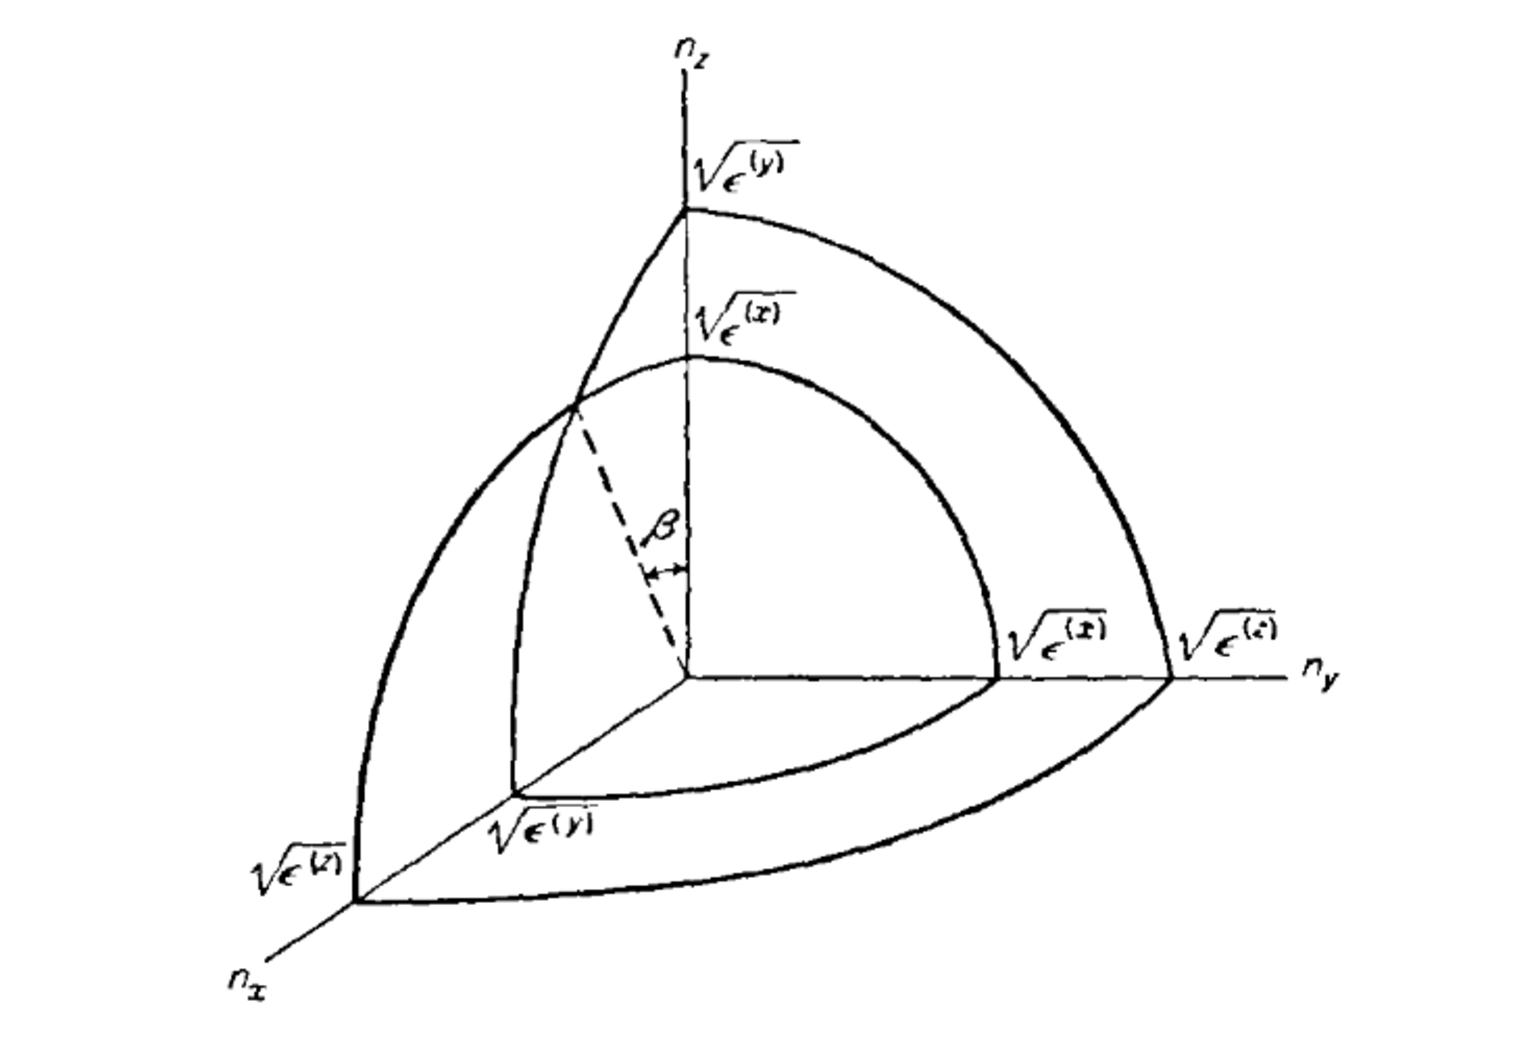
\includegraphics[width=\pltw]{figures/biaxial_ellipsoid.pdf}
\caption{Surface defined by Fresnel's equation for biaxial crystals.
    The lines are shown only on the planes parallel to the principle 
    axis of the crystal with $\eps_x < \eps_y < \eps_z$.
    The point of intersection defines the optical axis, 
    shown as a dashed line. 
    Taken from \cite{landau1984electrodynamics}. }
\label{fig:biaxial_ellipsoid}
\end{figure}
The optical axes are now defined by the straight lines intersecting 
the self intersects of the surface and the origin. 
Wave vector $\K$ and ray vector $\se$ have the same direction, 
only if they are orientated along one of the principle axes, 
otherwise they split up into two rays. 
Further, if $\K$ lies in one of the coordinate planes, so does $\se$.
There is, however an important exception: If the wave vector 
coincides with one of the optical axes, there are 
infinitely many ray vectors associated with it:
be can observe the phenomenon of 
\emph{internal conical refraction}. 
\FloatBarrier

\subsection{The electro-optic effect}
\paragraph{The index ellipsoid} 
as one of the two solutions for Fresnel's equation 
\eqref{eq:fresnel} for uniaxial crystals can be defined by the 
index ellipsoid, 
\begin{equation}
    \eta_{ij}^{(0)} n_i n_j = 1 \, ,
\end{equation}
where $\eta^{(0)} = {\eps^{(0)}}^{-1}$ is the \emph{impermeability 
tensor} of the unpertubed crystal with dielectric tensor $\eps^{(0)}$ 
and we sum over equal indices. 
Applying an electric field $\E$ on the crystal, $\eta^{(0)}$ will be 
changed to $\eta$. For reasonably small fields, we can expand
$\eta$ in powers of $\E$ as 
\begin{equation}
    \eta_{ij} = \eta_{ij}^{(0)} + r_{ijk} E_k + s_{ijkl} E_k E_l + \ldots
\end{equation}
The linear electro-optic effect is thus described by the 
\emph{electro-optic tensor} $r$, while 
$s$ is associtated with the quadratic electro-optic effect, etc. 
In this experiment, we will only look at effects of first order, 
since the associated second order \emph{Kerr effect} is 
neglectible for the given conditions~\cite{staatsexamen}.
Some basic properties of $r$ can be deduced immediately by 
looking at those of $\eps$: Since $\eps$ is real and symmetric, the 
same has to apply to $\eta$. Thus, $r$ has to be symmetric in the 
first two indices:
\begin{equation}
    r_{ijk} = r_{jik}
\end{equation}
We introduce a different notation as a $6 \times 3$ matrix with the definitions 
\begin{align}
    &r_{11k} = r_{1k}\, ,&
    &r_{22k} = r_{2k}\, ,&
    &r_{33k} = r_{3k}\, ,& \nonumber \\
    &r_{23k} = r_{32k} = r_{4k}\, ,& 
    &r_{13k} = r_{31k} = r_{5k}\, ,&
    &r_{12k} = r_{21k} = r_{6k} &
    \label{eq:notation}
\end{align}
for $k = 1, 2, 3$. The coefficient has a order of about 
$10^{-10}$ to $10^{-12}$ m/V.~\cite{sauter1996nonlinear}

\paragraph{The electro-optic tensor}
$r$ can be splitted into two components:
The \emph{primary} electro-optic effect with coefficient $r_{ij}'$
for the case of zero strain, where the crystal is 
not able to deform. The \emph{secondary} effect corresponds to deformation 
due to photoelastic and piezoelectric effects, described by the 
respective coefficients $d_{jk}$ and $p_{ik}$.
We can write
\begin{equation}
    r_{ij} = r_{ij}' + p_{ik} d_{jk}.
\end{equation}
In order to separate the effects, we apply an external field $\E$ 
oscillating at a frequency such that the crystal is not able 
to follow. In this case, the secondary electro-optical effect is surpressed, 
so we expect to measure $r'$. 

\subsection{Structure of crystals}

\subsubsection{Crystal systems}
\paragraph{Crystals can be categorized} 
into groups by their symmetries. 
There are three different categorizations in use, being 
partly equivalent and, accordingly introducing some confusion. 
The seven \emph{crystal system} divides crystals into 
according to the \emph{point group} of highest symmetry, 
the \emph{lattice system} 
categorizes according to the \emph{Bravais lattices}. While 
five of the crystal systems can be identified with five 
lattice systems, the hexagonal and trigonal crystal systems 
are different from the hexagonal and rhombohedral lattice systems. 
The \emph{crystal family} as a third categorization unifies 
the latter two and is thus made up of six elements. 

\paragraph{The lattice system} 
is based on the restrictions on the axial 
system, defined by the three 
\emph{primitive vectors} $\mathbf{a, b, c}$, which 
by the lattice translation operator 
\begin{equation}
    \mathbf{R} = n_1 \mathbf{a} + n_2 \mathbf{b} + n_3 \mathbf{c}
\end{equation}
define the \emph{Bravais lattice}. Each endpoint of a vector 
can be associated to one atom in the lattice of the crystal. 
Restricting only lenghts $a, b, c$ and angles $\alpha, \beta, \gamma$ 
between the primitive vectors, 
one obtaines the six crystal families, which by separating the 
family for $a = b \neq c, \alpha = \beta = 90^\circ, \gamma = 120^\circ$ 
into either hexagonal and trigonal system 
or hexagonal and rhombohedral system yields the crystal or lattice 
system, respectively. And overview is given in table 
\ref{tab:crystal_systems}. The hexagonal system is characterized by 
a sixfold rotational or rotoinversional symmetry, while the 
trigonal has a threefold rotational symmetry. 

\renewcommand{\arraystretch}{1.5}
\begin{table}[htdp]
    \begin{tabular}{|p{0.37\textwidth}|p{0.61\textwidth}|}
        \hline
        \rowcolor{LightCyan}
        $\textbf{Crystal system}$ & 
        $\textbf{Restrictions on the axial system   }$ \\ 
        \hline
        Trigonal        & $a \neq b \neq c; \quad \alpha = \beta = \gamma$ \\ 
        Monoclinic      & $a \neq b \neq c; \quad \alpha = \gamma = 90\Deg, \beta > 90\Deg$ \\ 
        Orthorhombic    & $a \neq b \neq c; \quad \alpha = \beta = \gamma = 90\Deg$         \\
        Tetragonal      & $a    = b \neq c; \quad \alpha = \beta = \gamma = 90\Deg$         \\ 
        Trigonal        & $a    = b \neq c; \quad \alpha = \beta = 90\Deg, \gamma = 120\Deg$ \\ 
        Hexagonal       & $a    = b \neq c; \quad \alpha = \beta = 90\Deg, \gamma = 120\Deg$ \\ 
        Cubic           & $a    = b =    c; \quad \alpha = \beta = \gamma = 90\Deg$         \\ 
        \hline
    \end{tabular}
\caption{
    The seven crystal systems, characterized by the restrictions on the axial system. 
    The trigonal and hexagonal systems are characterized by threefold and sixfold rotational 
    symmetries. 
    Reference: \cite{borchardt1995crystallography}
    }
\label{tab:crystal_systems}
\end{table}

\paragraph{Another characterization of crystals} 
can be done by the point groups. 
If we discard all lattice translations are discarded, we get 
a remaining set of symmetry operations on one of the lattice points, 
the so-called \emph{point group}. The symmetry operations $n, \bar{n}$ and $m$  
go through that point, while inversion ($\bar{1}$) is defined at the point. 
There are 32 point groups, which can be further ordered hierarchically to obtain 
the crystal groups. 
The space groups of highest symmetry for each crystal system is identified 
with one point group. As higher symmetries 
imply lower ones (e.~g. $4/m 2/m 2/m$ implies $2/m$), the lower 
symmetries often apply to several systems. However, the identification 
with the highest symmetry remains well defined. In table \ref{tab:point_groups}, 
we give an overview of the crystals and their associated point groups as 
well as subgroups.
The point groups are often named by 
the \emph{international} or \emph{Hermann-Mauguin notation} 
This convention allows to comprise all information about the point group in 
three symbols.
The notation follows the following rules~\cite{sands1993introduction}:
\begin{itemize}
    \item
    Each component corresponds to a different direction. 
    \item
    A number $n \in \mathbb{N}$ corresponds to a $n$-fold rotational symmetry 
    around the given axis. For crystals, $n$ is restricted to $1, 2, 3, 4, 6$.
    \item
    A number with an overbar $\bar{n}$ corresponds 
    to a rotoinversion as one operation. The special case $\bar{1}$ thus 
    means a simple inversion without rotation, i.~e. the existence of 
    an inversion center. 
    \item
    $m$ indicates a mirror plane, its direction is th normal to this plane.
    Terms written as $n/m$ thus indicate rotational symmetry and a mirror plane 
    normal to the axis of rotation, and are interpreted as one component. 
    \item
    For orthorhombic systems, all directions are mutually perpendicular. 
    The symbols refer to the $x$, $y$, and $z$ axis, respectively.
    \item
    For tetragonal systems, we chose the first component to be the $z$-axis, 
    with the symbol $4$ or $\bar{4}$. The second component refers to the 
    mutually perpendicular $x$- and $y$-axes and the third to directions in the 
    $xy$-plane bisecting the angles between $x$ and $y$. 
    \item
    In trigonal and hexagonal systems, the second component refers to 
    equivalent directions ($120^\circ$ or $60^\circ$ apart) in the $xy$-plane, 
    which is normal to the $z$-axis with $3, \bar{3}, 6$ or $\bar{6}$ symmetry. 
    \item
    For hexagonal systems, a third component corresponds to directions bisecting 
    the angles between axes specified by the second component. 
    \item
    If the second term is a $3$, then the system is cubic. The $3$ refers to the 
    four body diagonals of the cube, the first symbol refers to the cube axes, and the 
    third component to the face diagonals.
    \item
    If two or more axes coincide, the higher symmetry (generating more points) is 
    shown. 
\end{itemize}

\begin{table}[htdp]
    \begin{tabular}{|p{0.37\textwidth}|p{0.23\textwidth}|p{0.37\textwidth}|}
        \hline
        \rowcolor{LightCyan}
        $\textbf{Crystal system}$ & 
        \multicolumn{2}{|l|}{$\textbf{Point groups   }$} \\ 
        \cline{2-3}
        \rowcolor{LightCyan}
        &$\textbf{Highest symmetry }$ & $\textbf{subgroups}$\\ 
        \hline
        Trigonal        & $ \bar{1} $   & $ 1 $  \\ 
        Monoclinic      & $\frac{2}{m}$ & $m, 2$     \\ 
        Orthorhombic    & $\frac{2}{m} \frac{2}{m} \frac{2}{m}$ & $mm2, 222$     \\
        Tetragonal      & $\frac{4}{m} \frac{2}{m} \frac{2}{m}$ & $\bar{4}2m, 4mm, 422, \frac{4}{m}, \bar{4}, 4$     \\ 
        Trigonal        & $\bar{3} \frac{2}{m}$         & $3m, 32, \bar{3}, 3$      \\ 
        Hexagonal       & $\frac{6}{m} \frac{2}{m} \frac{2}{m}$ & $\bar{6}m2, 6mm, 622, \frac{6}{m}, \bar{6}, 6$     \\ 
        Cubic           & $\frac{4}{m}\bar{3}\frac{2}{m}$ & $\bar{4}3m, 432, \frac{2}{m}\bar{3}, 23 $     \\ 
        \hline
    \end{tabular}
\caption{
    Point groups, their subgroups and associated crystal systems, 
    written in the \emph{international notation}.
    Reference: \cite{borchardt1995crystallography}
    }
\label{tab:point_groups}
\end{table}

\paragraph{The $\bar{4}2m$-symmetry}
under consideration in this experiment corresponds to 
\begin{itemize}
    \item
    a fourfold rotoinversional symmetry around the $x_3$-axis
    \item
    a twofold rotational symmetry around the $x_1$-axis
    \item
    and a mirror plane parallel to the $x_3$-axis and the bisection of the 
    angles between $x_1$- and $x_2$-axis, 
\end{itemize}
where we renamed the axes $x, y$ and $z$ into $x_1, x_2$ and $x_3$, respectively. 
The $\bar{4}$-axis includes another mirror 
plane perpendicular to the first one and a twofold rotational symmetry 
around the $x_3$-axis. 
The structure is usually called tetragonal scalenohedral. 

\paragraph{Point groups can further} 
be illustrated by their \emph{stereographic projections},
that is constructed as follows
~\cite{borchardt1995crystallography}: 
We take the plane going through the origin 
of the point group and being perpendicular to the axis of highest 
symmetry to be the plane of projection. We further construct a sphere 
of arbitry radius and draw straight lines from the origin through the 
centers of the crystal's faces. If we take all intersections of these lines 
with the surface of the upper hemisphere and draw lines to the south pole, 
the intersects with the projection plane give the desired stereographic projection. 
The process is illustrated in the figures \ref{fig:stereo}. 
The projection can then be further reduced to the \emph{assymetric face unit}, 
which is the smallest unit of surface of the sphere, which will generate 
the entire sphere by application of all symmetry operations
~\cite{borchardt1995crystallography}.
For the $\bar{4}2m$-crystals, both the stereogram and the asymmteric face unit are 
shown in figure \ref{fig:stereo_42m}.

\begin{figure}[h]
    \begin{subfigure}[b]{\picwidth}
    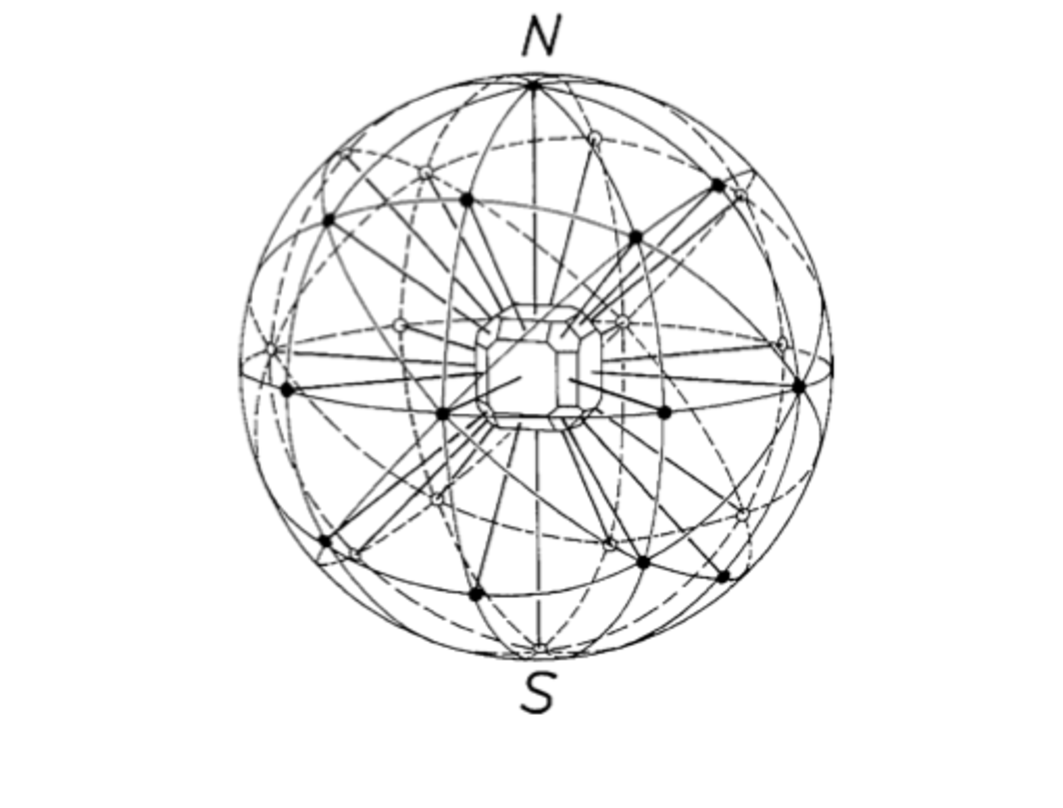
\includegraphics[width=\textwidth]{figures/stereo_1}
    \caption{}
    \label{fig:stereo_1}
    \end{subfigure}\qquad
    \begin{subfigure}[b]{\picwidth}
    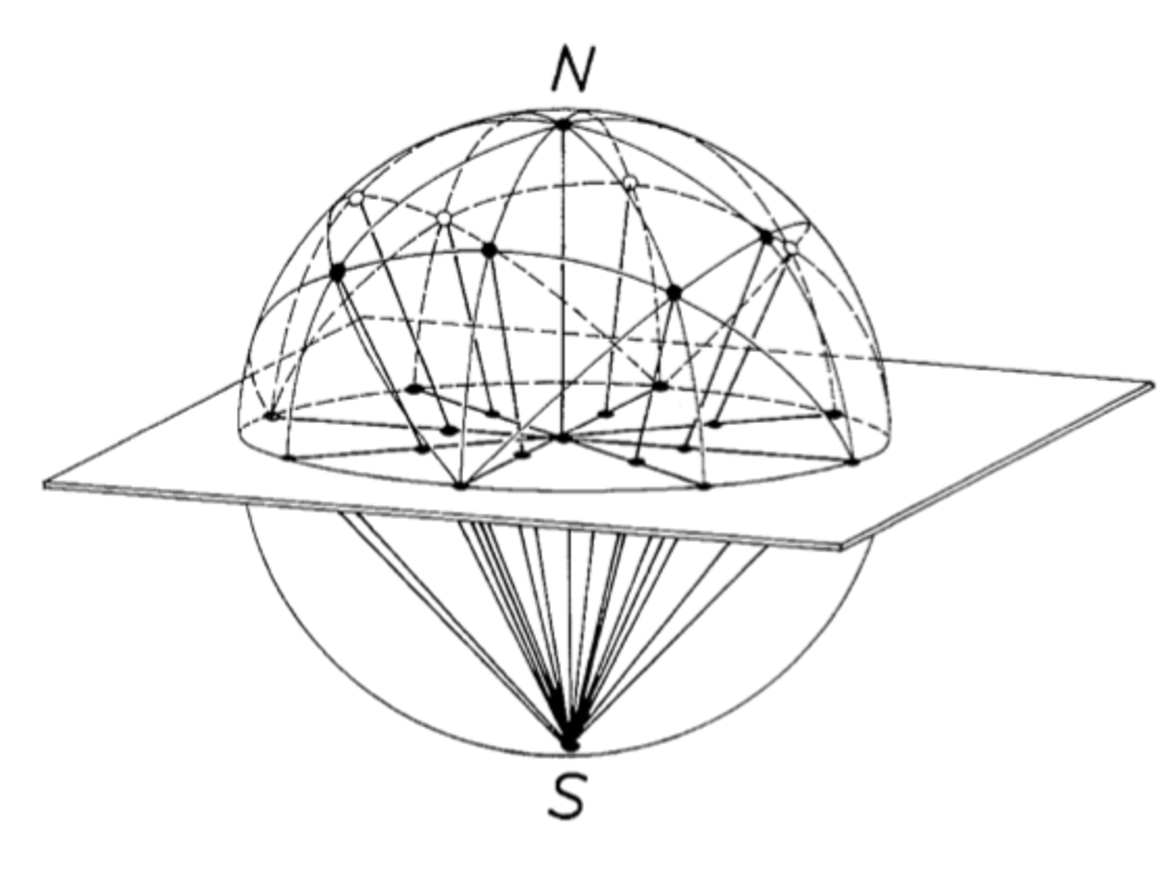
\includegraphics[width=\textwidth]{figures/stereo_2}
    \caption{}
    \label{fig:stereo_2}
    \end{subfigure}
    \begin{subfigure}[b]{\picwidth}
    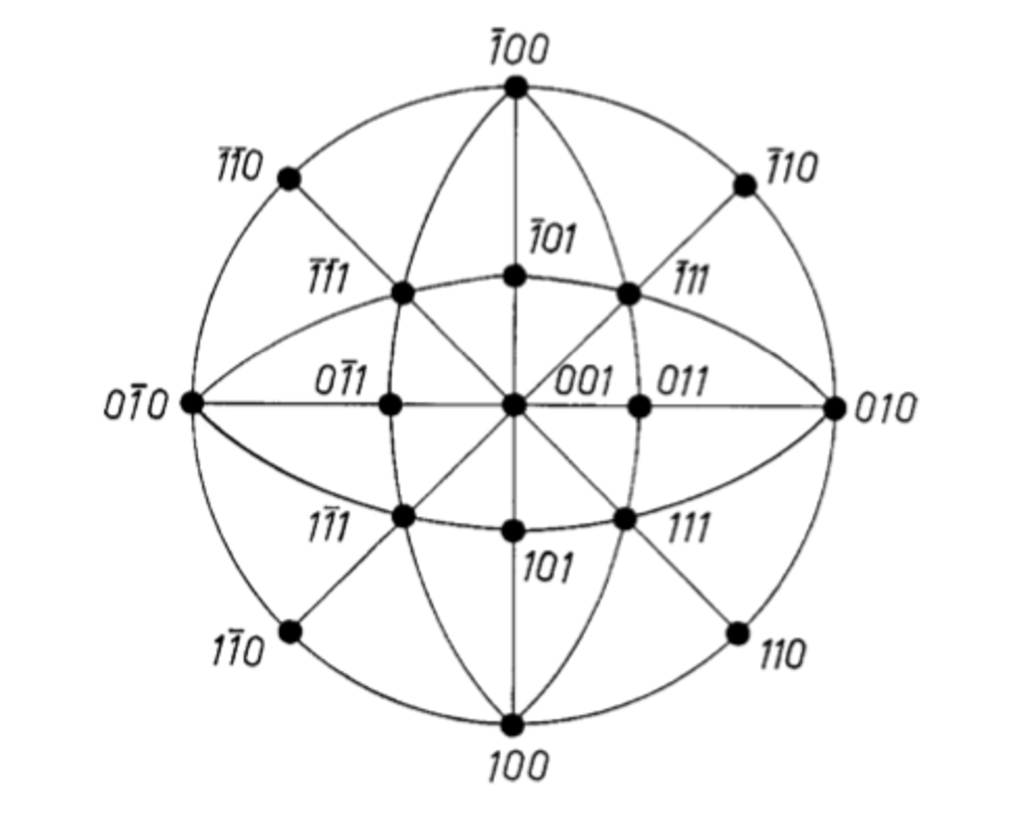
\includegraphics[width=\textwidth]{figures/stereo_3}
    \caption{}
    \label{fig:stereo_3}
    \end{subfigure}
    \caption{
        Illustration of the stereographic projection:\\
        \ref{fig:stereo_1}:
            Crystal at the center of the sphere with points of intersections, 
            here shown for galena (PbS).
        \ref{fig:stereo_2}:
            Construction of the projection with the 
            plane of projection and south pole.
        \ref{fig:stereo_3}:
            Result of stereographic projection for PbS. The lines 
            show the interconnecting great circles projected on the plane. 
            All figures taken from~\cite{borchardt1995crystallography}.}
    \label{fig:stereo}
\end{figure}

\begin{figure}
    \centering
    \begin{subfigure}[b]{0.36\textwidth}
    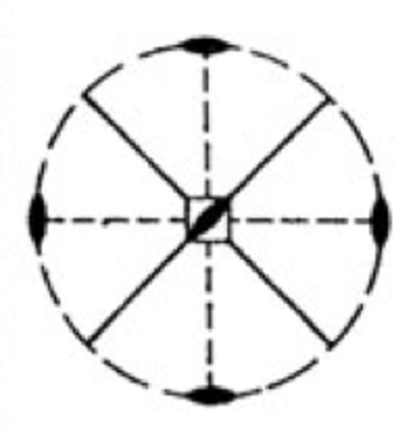
\includegraphics[width=\textwidth]{figures/stereogram_42m}
    \caption{}
    \label{fig:stereogram_42m}
    \end{subfigure}\qquad
    \begin{subfigure}[b]{0.45\textwidth}
    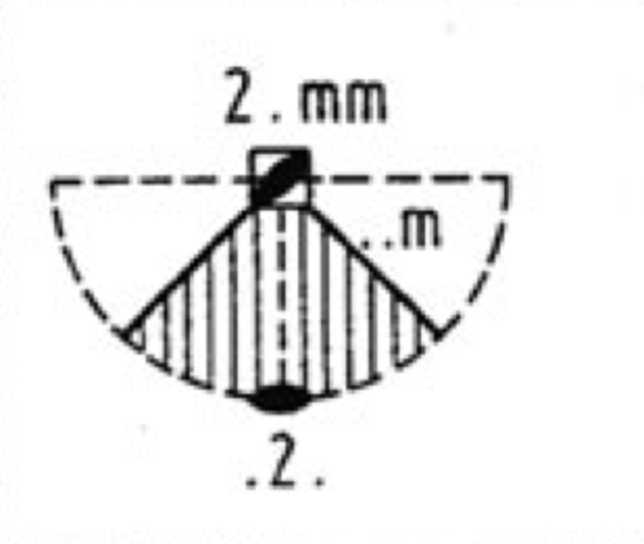
\includegraphics[width=\textwidth]{figures/asym_face_unit_42m}
    \caption{}
    \label{fig:asym_face_unit_42m}
    \end{subfigure}
    \caption{
        Stereogram (\ref{fig:stereogram_42m}) and asymmetric face unit
        \ref{fig:asym_face_unit_42m} of the $\bar{4}2m$ point group,
        to which the ADP crystal used in this experiment belongs. 
        The symbols are 
        defined as follows: The square with diagonal corresponds 
        to the fourfold rotoinversion axis $\bar{4}$ perpendicular 
        to the plane, the small oval to the twofold rotation axis 
        $2$, which lies in the plane. The solid line at $45\Deg$
        corresponds to the mirror plane $m$. 
        Application of all symmetry operations on the shaded area 
        yield the entire stereographic projection. 
        Taken from~\cite{borchardt1995crystallography}.
        }
    \label{fig:stereo_42m}
\end{figure}



\FloatBarrier

\subsubsection{Optical classification of crystals}
\label{sec:optical_axes}
Crystals can be classified into three groups according to their 
optical properties~\cite{born1999principles}. 
\begin{itemize}
    \item 
    Group I - \emph{Isotropic crystals}:\\
    Crystals of the cubic system, for which $\eps_{ij} = \eps \delta$, and 
    $\eps$ is a scalar, meaning that three crystallographically 
    equivalent and mutually perpendicular axes can be chosen freely. 
    Optically, these crystals are equivalent to isotropic bodies. 
    \item
    Group II - \emph{Uniaxial crystals}: \\
    Crystals not belonging to group I, but for which one can choose 
    two or more crystallographically equivalent axes in a plane. 
    These crystals are in the rhobohedral, tetragonal or hexagonal system. 
    The optical axes coincides with the threefold, 
    fourfold or sixfold axis of symmtry, respectively, while the 
    other two axes arbitrary
    \item
    Group III - \emph{Biaxial crystals}: \\
    Crystals in which no two crystallographically equivalent axes may 
    be chosen, belonging to the triclinic, monoclinic, or orthorhombic 
    system. For the triclinic crystals, principla dielectric axes are 
    unrelated to the crystallographic  axes and vary with frequency. 
    For monoclinic ones, only one principle dielectric axis is crystallographically 
    fixed. It coincides with the twofold axes of symmetry, 
    or is perpendicular to the plane of symmetry, while other two axes 
    vary with frequency. 
    In orthorhombic crystals, all three principly dielectric axes are fixed. 
    They coincide with three mutually perpendicular twofold axes of symmetry.
\end{itemize}
A survey of all possible case is given in table \ref{fig:crystal_ellipsoid}.
\begin{table}
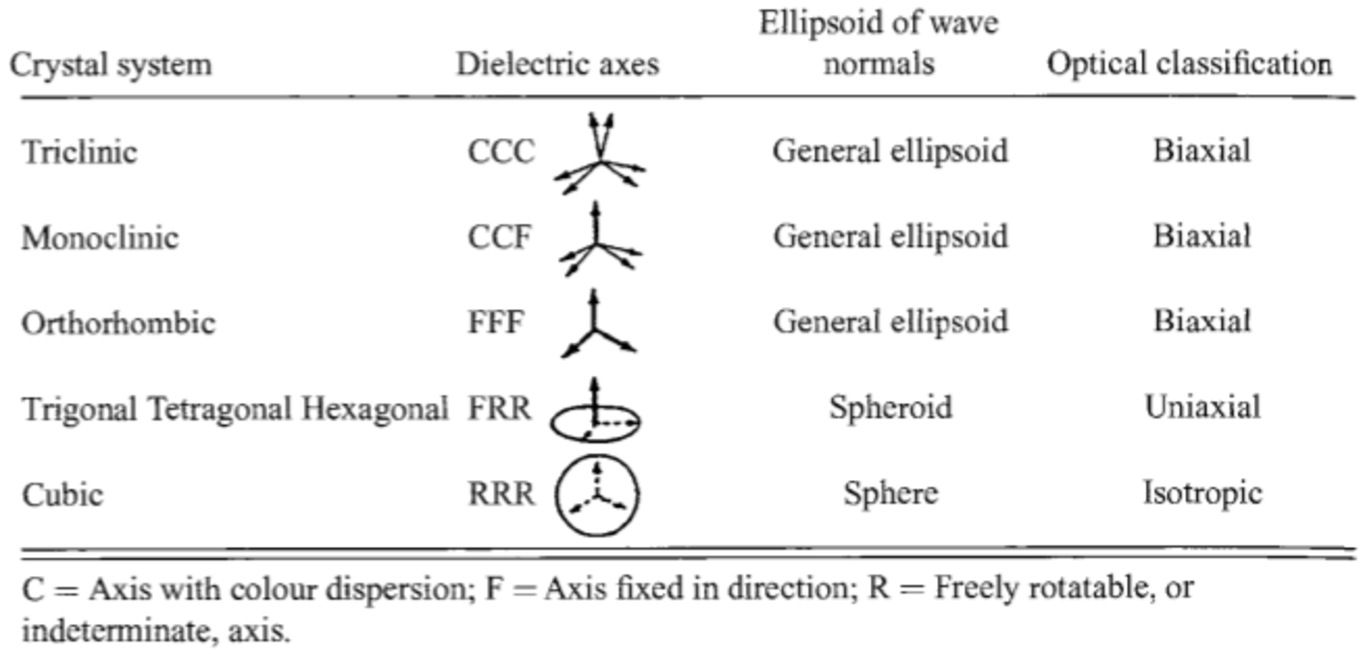
\includegraphics[width=\pltw]{figures/crystal_ellipsoid.pdf}
\caption{
    Table summarizing the optical properties of crystals, grouping them 
    according to the principle axes of the dieletric tensor $\eps$. 
    Two vectors at a small angle are indicating frequency-dependency 
    of the correspoding principle axes (signifying positions for two different 
    frequencies/colours). Axes that can be rotated freely in a plane are represented 
    by dashed vectors. 
    From \cite{born1999principles}. }
\label{fig:crystal_ellipsoid}
\end{table}

\FloatBarrier

\subsection{Reduction of Dielctric tensor}
\label{sec:reduce}
\paragraph{As described in} 
the previous section, the ADP-crystal has the symmetry group 
$\bar{4}2m$. We can reduce the number of non-zero components of the 
electro-optic tensor $r_{ijk}$ by the following consideration:
If we apply a coordinate transform $R$ to our basis for which 
our crystal is symmetric, then $r_ijk$ has to have the same symmetry, 
i.~e. the repsresentation of $r_ijk$ in the new basis has to be the same.
We define $R$ with its action on the basis by 
\begin{equation}
    \mathbf{\hat{e}}_i = R_i^j \mathbf{e}_j \, ,
\end{equation}
where $\mathbf{\hat{e}}_i$ and $\mathbf{e}_i$ are 
the $i$-th components of the new and old basis, respectively. 
Since $r_{ij}$ is a tensor, the components $\hat{r}_{ijk}$ in the 
new basis can be calculated from those in the old one by 
\begin{equation}
    \hat{r}_{ijk} = 
        \left( R^{-1}\right)_i^l
        \left( R^{-1}\right)_j^m
        \left( R^{-1}\right)_k^n
        r_{lmn} \, .
\end{equation}


\paragraph{Before applying the symmetries}
of the crystal under consideration 
we make one general observation: Crystals with an inversion 
center are not subject to either the Pockels effect. 
This can be deduced as follows:
As a center of inversion means symmetry under the transformation 
\begin{equation}
    \begin{split}
    x_1 &\rightarrow -x_1 \\
    x_2 &\rightarrow -x_2 \\
    x_3 &\rightarrow -x_3  \, ,
    \end{split}
\end{equation}
all components in the new bases $\hat{r}_{ijk}$ will be defined 
by 
\begin{equation}
   \hat{r}_{ijk} = - r_{ijk}.
\end{equation}
But symmetry implies equality. Thus all components have to be zero. 
The same reasoning applies to other effects with a similar mathematical 
structure, such as the piezoelectric effect. 


\paragraph{Returning to the} $\bar{4}2m$ group, 
we eliminate the components of $r_{ijk}$ by applying sequentially 
the following transformations, for which the crystal is symmetric:
\begin{itemize}
    \item
    rotation by $180^\circ$ around the $x_3$-axis;
    \item
    rotation by $90^\circ$ around the $x_3$-axis and inversion;
    \item
    rotation by $180^\circ$ around the $x_1$-axis. 
\end{itemize}
For the first rotation, the coordinates transfer with 
\begin{equation}
    \begin{split}
    x_1 &\rightarrow -x_1 \\
    x_2 &\rightarrow -x_2 \\
    x_3 &\rightarrow x_3  \, .
    \end{split}
\end{equation}
The matrix representation is given by
\begin{equation}
    R^{-1} = 
    \begin{pmatrix}
    -1 &  0 &  0 \\
     0 & -1 &  0 \\
     0 &  0 &  1 
    \end{pmatrix} \, .
\end{equation}
We calculate the first component in an examplary manner, 
\begin{equation}
    \begin{split}
    \hat{r}_{111} &= 
        \left( R^{-1}\right)_1^l
        \left( R^{-1}\right)_1^m
        \left( R^{-1}\right)_1^n
        r_{lmn}  \\
        &= (-1)(-1)(-1)r_{111} \\
        &= -r_{111} \, .
    \end{split}
\end{equation}
One can see immediately that for all components an odd number 
of indices $i \in \{1, 2\}$ yields $\hat{r}_{ijk} = -r_{ijk}$, 
while an even number yields $\hat{r}_{ijk} = r_{ijk}$. 
Since the condition of symmtry implies $\hat{r}_{ijk} = r_{ijk}$, 
we can summarize all components which do not have to equal zero:
\begin{align}
    &{r}_{113}\, ,& 
    &{r}_{123} = {r}_{213}\, , &
    &{r}_{231} = {r}_{321}\, , \nonumber \\ 
    &{r}_{223}\, ,& 
    &{r}_{131} = {r}_{311}\, , & 
    &{r}_{232} = {r}_{322}\, , \nonumber \\ 
    &{r}_{333}\, ,& 
    &{r}_{132} = {r}_{312}
\end{align}
A rotation by $90^\circ$ around the  
$x_3$ axis and following 
inversion is given by the coordinate transformation 
\begin{equation}
    \begin{split}
    x_1 &\rightarrow -x_2  \\
    x_2 &\rightarrow x_1 \\
    x_3 &\rightarrow -x_3  \, .
    \end{split}
\end{equation}
with the matrix representation
\begin{equation}
    R^{-1} = 
    \begin{pmatrix}
    0 & -1 &  0 \\
    1 &  0 &  0 \\
    0 &  0 & -1 
    \end{pmatrix} \, .
\end{equation}
Applying ths transformation to the remaining components yields:
\begin{align*}
    \hat{r}_{123} &=  r_{213} \, ,&  
    \hat{r}_{213} &=  r_{123} \, , \\
    \hat{r}_{132} &=  r_{231} \, ,&    
    \hat{r}_{231} &=  r_{132} \, , \\
    \hat{r}_{312} &=  r_{321} \, ,&   
    \hat{r}_{321} &=  r_{312} \, , \\
    \hat{r}_{113} &= -r_{223} \, ,&  
    \hat{r}_{223} &= -r_{113} \, , \\
    \hat{r}_{131} &= -r_{232} \, ,&  
    \hat{r}_{232} &= -r_{131} \, , \\
    \hat{r}_{311} &= -r_{322} \, ,&  
    \hat{r}_{322} &= -r_{311} \, , \\
    \hat{r}_{333} &= -r_{333} \,         % !
\end{align*}
We see, that only $r_{333}$ has to vanish, while further 
equalities are introduced. 
To further reduce the number, we  apply the rotation by 
$180^\circ$ around the $x_1$-axis, given by 
\begin{equation}
    \begin{split}
    x_1 &\rightarrow x_1  \\
    x_2 &\rightarrow -x_2 \\
    x_3 &\rightarrow -x_3 \\
    \end{split} \ ; \qquad
    R^{-1} = 
    \begin{pmatrix}
    1 &  0 &  0 \\
    0 & -1 &  0 \\
    0 &  0 & -1 
    \end{pmatrix} \, .
\end{equation}
Since $R^{-1}$ is diagonal, the indices remain the same, thus 
components with changing sign have to vanish. This is the case 
only for an those triples of indices with an 
odd number of indices $i \in \{2, 3\}$. We conclude, that 
the remaining components with corresponding equalities are given by
\begin{align*}
    r_{123} &=  r_{213}\, , \\
    r_{132} &=  r_{312} = r_{231} = r_{321}\,
\end{align*}
These can be renamed in the way given by equations \eqref{eq:notation}, 
which leaves only the three remaining components
\begin{equation}
    r_{41} = r_{52} \qquad \text{ and } \qquad  r_{63}\, .
\end{equation}

\subsection{Application to Pockels Cell}
\label{sec:application_cell}
By applying the result of the foregoing discussion, we can significantly 
reduce the parameters in questions for the pertubed index ellipsoid
\eqref{eq:B_ij}. We resume the most important results:
\begin{itemize}
    \item
    Without the external field, the crystal is uniaxial 
    (refer to section \ref{sec:optical_axes}).
    \item
    We chose the principle dielectric axis system. The 
    components of $\eps$ are named $\eps_\perp$ and 
    $\eps_\parallel$ as defined in equations 
    \eqref{eq:eps_perp} and \eqref{eq:eps_parallel}.  
    \item
    Optical axis and $\bar{4}$-axis coincide. We define 
    this axis to be the $x_3$-axis. Thus, the 
    only non-zero components of the electro-optic tensor 
    $r_{ij}$ are $r_{41} = r_{52}$ and $r_{63}$ in the 
    chosen coordinates, as described in the previous section 
    \ref{sec:reduce}
\end{itemize}


Inserting these conditions in the index generalized index ellipsoid 
\eqref{eq:ellipsoid_pertubed}, 
we arrive at the defining equation
\begin{equation}
    \frac{1}{\eps_\perp}\left(n_1^2 + n_2^2\right) + 
    \frac{1}{\eps_\parallel} n_3^2 + 
    2 r_{41} \left(E_1 n_2 + E_2 n_1\right)n_3 + 
    2 r_{63} E_3 n_1 n_2  = 1\, ,
    \label{eq:ellipsoid_red}
\end{equation}
where, as before, the wave vectors $\K$ are related to 
$\N$ by \eqref{eq:def_n}. 
The Pockels Cell used in this experiment is a transverse one, 
thus the $\E$-field is applied in direction of $x_1$, e.~i. 
$E_2 = E_3 = 0$. This yields
\begin{equation}
    \frac{1}{\eps_\perp}\left(n_1^2 + n_2^2\right) + 
    \frac{1}{\eps_\parallel} n_3^2 + 
    2 r_{41} E_1 n_2 n_3  = 1 \, .
    \label{eq:ellipsoid_trans}
\end{equation}
The crystal is aligned with a $45^\circ$-Y-cut. In order to 
use the laboratory frame as coordinate system, we rotate our 
coordinate system by $45^\circ$ around the $x_1$-axis, 
after which the components of $\N$ read
\begin{align}
    n_1 &= n_1'  \\
    n_2 &= \frac{1}{\sqrt{2}}\left(n_2' + n_3'\right) \\
    n_3 &= \frac{1}{\sqrt{2}}\left(n_2' - n_3'\right) \, .\\
    \label{eq:trans_ycut}
\end{align}
Equation \eqref{eq:ellipsoid_trans} then becomes
\begin{align}
    1 &= 
    \frac{1}{\eps_\perp}
    \left[ {n_1'}^2 + 
    \frac{1}{2} \left({n_2'}^2 + {n_3'}^2 \right) + 
    {n_2'}{n_3'} \right] + 
    \frac{1}{\eps_\parallel}
    \left[\frac{1}{2} \left({n_2'}^2 + {n_3'}^2 \right) -  
    {n_2'}{n_3'} \right] + 
    r_{41} E_1 \left({n_2'}^2 - {n_3'}^2\right) 
    \nonumber \\
    &= 
    \frac{1}{\eps_\perp} {n_1'}^2 + 
    \frac{1}{2} \left(\frac{1}{\eps_\perp} + \frac{1}{\eps_\parallel}\right)
    \left({n_2'}^2 + {n_3'}^2 \right) + 
    \left( \frac{1}{\eps_\perp} - \frac{1}{\eps_\parallel}\right)
    {n_2'}{n_3'}  + 
    r_{41} E_1 \left({n_2'}^2 - {n_3'}^2\right) 
    \nonumber \\
    &= 
    \frac{1}{\eps_\perp}  {n_1'}^2 + 
    {n_2'}^2 \left(\frac{1}{\eps_x} + r_{41} E_1 \right) +
    {n_3'}^2 \left(\frac{1}{\eps_x} - r_{41} E_1 \right) +
    {n_2'}{n_3'} \left( \frac{1}{\eps_\perp} - \frac{1}{\eps_\parallel}\right) \, ,
    \label{eq:ell_calc}
\end{align}
where we defined 
\begin{equation}
    \frac{1}{\eps_x} := 
    \frac{1}{2} \left( \frac{1}{\eps_\perp} + \frac{1}{\eps_\parallel}\right) \, .
    \label{eq:def_eps_x}
\end{equation}
We observe, that the main axes of the ellipsoid are no longer parallel to the 
crystal's princial axes.
For the experiment, we rely on polarized beams. For a ray with 
$\K$ in the $x_2'$-direction, polarized in the area bisecting the 
$x_1'$- and $x_3'$-axis, the component $n_2'$ vanishes.
Equation \eqref{eq:ell_calc} then reduces to
\begin{equation}
    1 = \frac{1}{\eps_\perp}  {n_1'}^2 + 
    {n_3'}^2 \left(\frac{1}{\eps_x} - r_{41} E_1 \right) \, .
    \label{eq:ell_02}
\end{equation}
The wave splits up into two rays, one polarized in $x_1'$-, 
the other in $x_3'$-direction. Accordingly, they experience the refraction 
\begin{align}
    n_1' &= \sqrt{\eps_\perp} 
    \label{eq:n1p} \\
    n_3' &= \frac{\sqrt{\eps_x}}{\sqrt{1 - r_{41} E_1 \eps_x}}
    \label{eq:n3p} 
\end{align}
In order to facilitate the result, we do a scale analysis for the 
parameters of the given Pockels Cell, which are stated in the 
section describing the experimental setup \ref{sec:setup_pockels}.
With $n = \sqrt{\eps / \epsn}$, we get $\eps_x / \epsn \sim 1$, for 
a voltage of $U = 240$V, $E = U / d \sim 10^5$V/m, 
so we can approximate $r_{41} E_1 \eps_x / \epsn \sim 10^{-6}$. 
We can thus expand \eqref{eq:n3p} to the first order in $E_1$ and 
obtain
\begin{equation}
    n_3' \approx \sqrt{\eps_x} + 
        \frac{1}{2} r_{41} E_1 {\eps_x}^\frac{3}{2}
    \label{eq:n3paprrox} \, .
\end{equation}
For the phase difference of the two components after passing through a crystal 
of length $l$, we get with \eqref{eq:dphi}:
\begin{equation}
    \begin{split}
    \Delta \phi_1 
    &= \frac{2l \pi}{\lambda} \left(n_3' - n_1' \right) \\
    &= \frac{l \pi}{\lambda}\Bigg[
    \underbrace{r_{41} E_1 {\eps_x}^\frac{3}{2}}_\text{Pockels effect} + 
    \underbrace{2\left(\sqrt{\eps_x} - \sqrt{\eps_\perp} 
    \right)}_\text{natural birefraction}
    \Bigg]
    \end{split}
    \label{eq:dphi_1}
\end{equation}
In order to reunited the beams that are split up by the Pockels effect, 
we let the beam pass another crystal and corresponding $\E$-field 
turned around together by $180^\circ$. 
Since the situation is symmetric for the phase difference, we get for the 
\begin{equation}
    \Delta \phi_2 = \Delta \phi_1
\end{equation}
resulting phase difference  
The second summand in \eqref{eq:dphi_1} corresponds to the natural birefringence. 
It can be cancelled out by applying another pair of crystals turned by 
$90^\circ$ towards the first one. In this case, the beam polarized 
in the former $x_1'$-direction is subject to the refractive index 
$n_3'$ and vice versa. In order to not cancel the part depending on $\E$, 
the field has to be turned around with respect to the new coordinates. 
The phase difference is then given by 
\begin{equation}
    \begin{split}
    \Delta \phi_3 = \Delta \phi_4
    &= \frac{2l \pi}{\lambda} \left(n_1' - n_3' \right) \\
    &= -\frac{l \pi}{\lambda}\left[
    r_{41} (-E_1) {\eps_x}^\frac{3}{2} + 
    2\left(\sqrt{\eps_x} - \sqrt{\eps_\perp}
    \right)
    \right]
   \end{split}
    \label{eq:dphi_34}
\end{equation}
Adding all phase differences yields
\begin{equation}
    \begin{split}
    \Delta \phi_\mathrm{total}  
    &= \Delta \phi_1 + \Delta \phi_2 + \Delta \phi_3 + \Delta \phi_4 \\
    &= \frac{4l \pi}{\lambda} r_{41} E_1 {\eps_x}^\frac{3}{2} 
    \end{split}
    \label{eq:dphi_34}
\end{equation}
At $\Delta \phi = \pi$, the Pockels Cell acts as a \emph{half-wave plate}. 
In this case, light will pass through orthogonally oriented polarizers 
with the cell in between entirely only for the correspoding $\E_{\lambda/2}$,
while for $\E = 0$, no light is transmitted. Using $E = U / d$, we can thus 
define $U_{\lambda / 2}$ and use the setup to measure the electro-optic 
coefficient 
\begin{equation}
    r_{41} = \frac{\lambda d}{4 l U_{\lambda / 2}} 
    \left(\frac{1}{2} \left(\frac{1}{\eps_\perp} + \frac{1}{\eps_\parallel}\right)\right)^{\frac{3}{2}}
    \label{eq:r_41_U}
\end{equation}


\clearpage
\section{Experimental setup for Pockels effect}
\subsection{Setup}
\label{sec:setup_pockels}
The experimental setup consists of the beam bath with the Pockels Cell, 
two polarizators and a photodiode as well as the signal generating and 
analysing electronics. The beam is produced by a HeNe laser operating in 
the red part of the visualspectrum and guaranteeing monocromatic light 
at 632.8nm in air~\cite{versuchsanleitung}. 

A block diagram of the setup is given in figure \ref{fig:setup_block}, 
the actual instruments are shown in the photo \ref{fig:setup_photo}. 
\begin{figure}
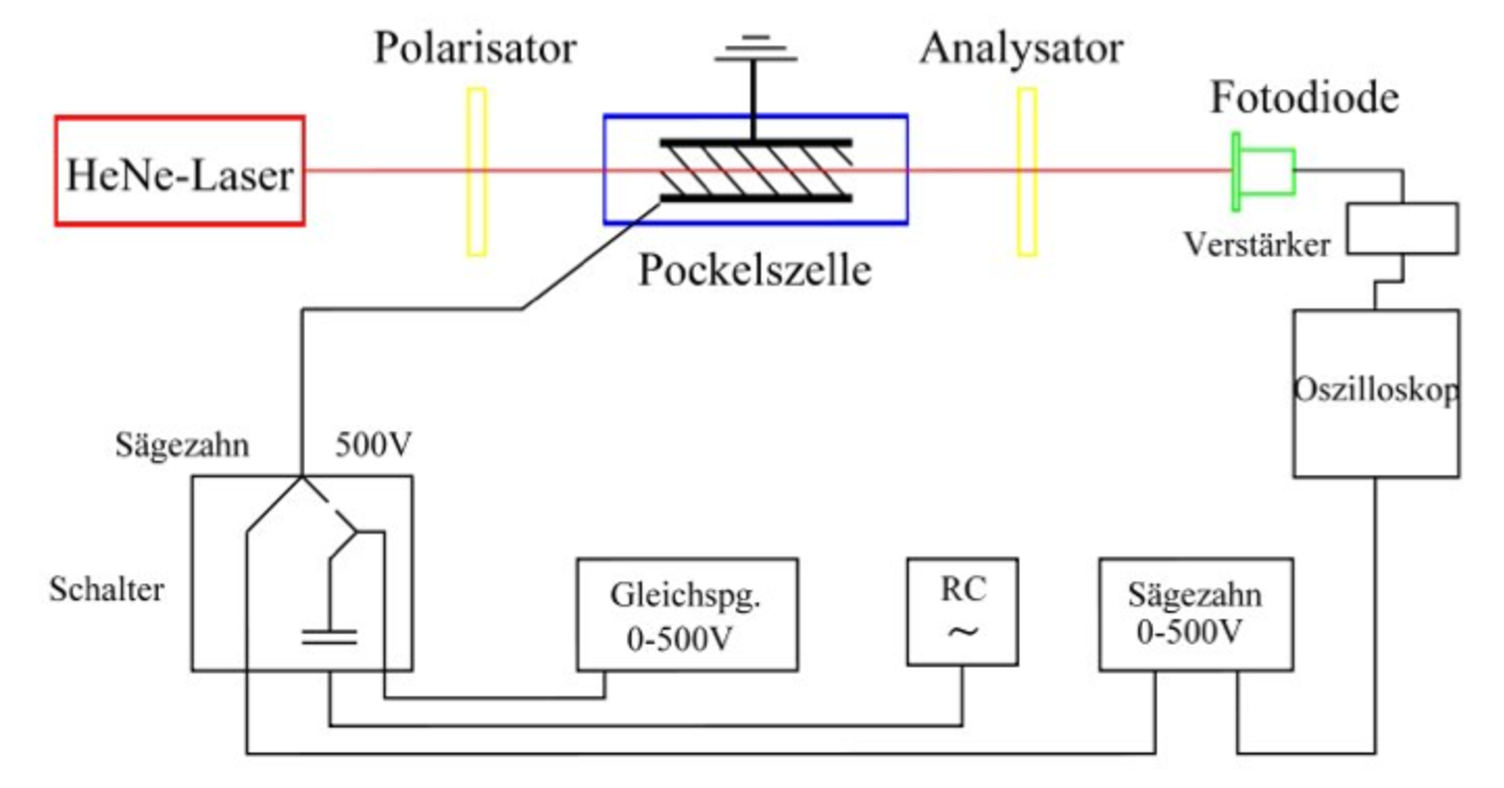
\includegraphics[width=\pltw]{figures/setup_block.pdf}
\caption{
    Block diagram of the experimental setup for measuring the 
    Pockels effect, 
    from~\cite{versuchsanleitung}.
    }
\label{fig:setup_block}
\end{figure}
\begin{figure}
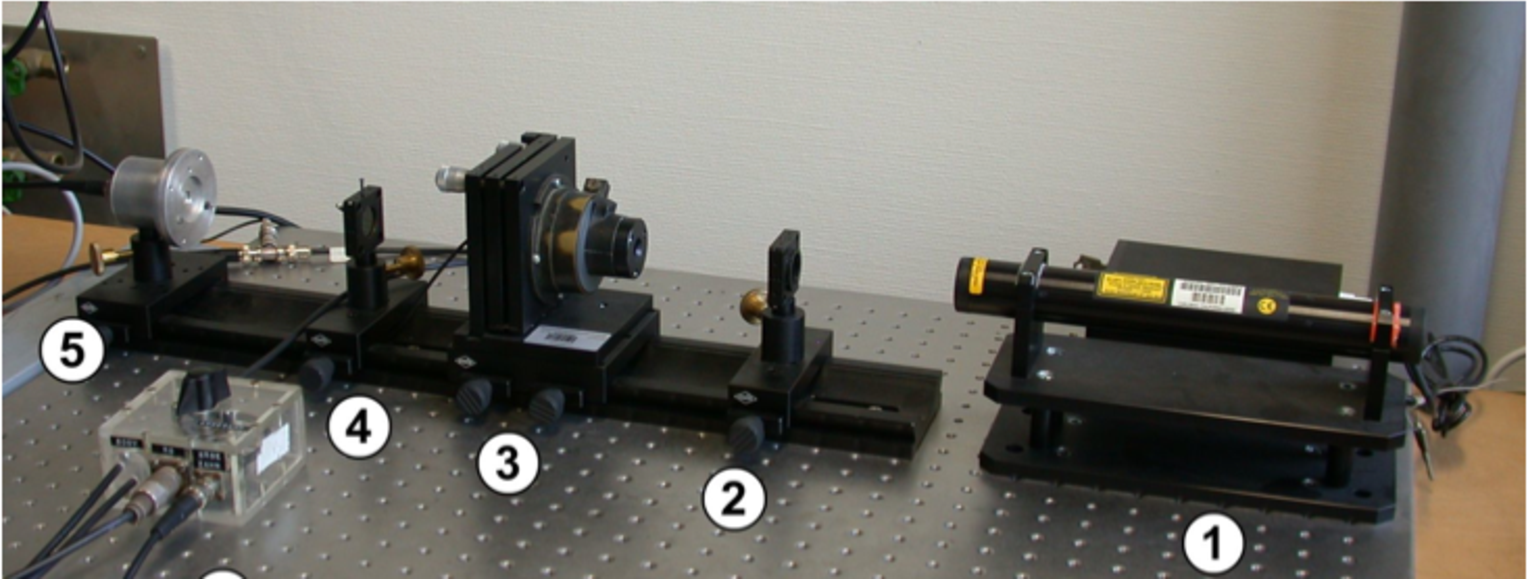
\includegraphics[width=\textwidth]{figures/setup_photo.pdf}
\caption{
    Photo of the experimental setup for measuring the 
    Pockels effect with the following devices:
    1) He-Ne-Laser, 2) polarisator, 3) Pockels Cell, 
    4) analysator, 5) photodiode;
    modified from~\cite{versuchsanleitung}.
    }
\label{fig:setup_photo}
\end{figure}
The Pockels Cell consists of four ADP crystals aligned in the beam path, 
as shown in figure \ref{fig:pockels_cell_path}.
\begin{figure}
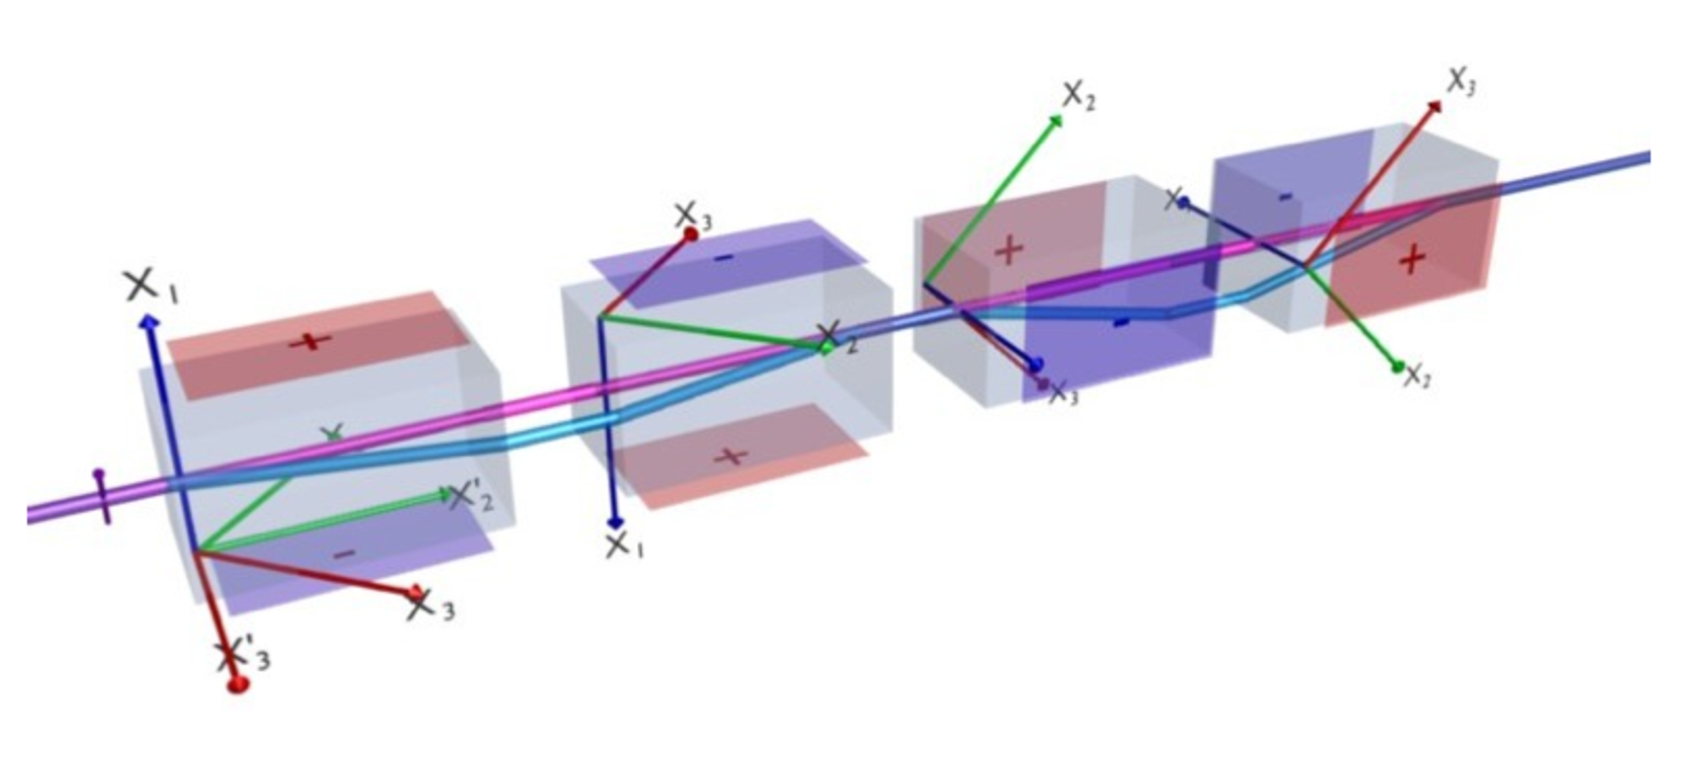
\includegraphics[width=\textwidth]{figures/pockels_cell_path.pdf}
\caption{
    Alignment of crystals of the Pockels Cell. One can the the different 
    rotations of the crystals and the applied electric fields 
    relative to each other, cancelling the separation of beams and 
    natural double refraction. The birefringence of 
    the beam path is shown schematically with the blue and violet beam. 
    From~\cite{versuchsanleitung}.
    }
\label{fig:pockels_cell_path}
\end{figure}
The eletric fields are applied by condensators with the plates 
orientated perpendicular to the $x_1$ axis of the crystal in 
it's principle dieletric axes system, which implies, that the 
$x_3$ axis of fourfold rotoinversion is parallel to the condensator 
plates. As elaborated in the theoretical section, this 
setup corresponds to the \emph{transverse Pockels effect}. 
All crystals are prepared in the $45\Deg$-Y-cut relative to the crystal 
lattice. The light thus enters in the direction of the line 
bisecting the $x_3$ and $x_2$ axis of the crystal. This direction 
is named $x_2'$. 
In order to annul the separation of the arising two beams, 
the first two and the second two crystals and their condensators 
are rotated by $180\Deg$ one to another. The second pair is 
further rotated by $90\Deg$ and has it's electric field inverted, 
such that the naturally arising birefringence is cancelled. 

The parameters of the used Pockels cell are shown in 
table \ref{tab:pockels_technical}.

\begin{table}[htdp]
    \begin{tabular}{|p{0.61\textwidth}|p{0.37\textwidth}|}
        \hline
        Number of crystals & 4 \\
        Crystal cut & $45\Deg$-Y-cut \\
        Wavelenght of HeNe Laser & 632.8 nm \\
        Thickness of crystall & $d = 2.4$ mm \\
        Refractive index in $x_1$ and $x_2$ direction & $n_1 = 1.522$  \\
        Refractive index in $x_3$ direction & $n_3 = 1.477$  \\
        Electro-optic coefficient & $r_{41} = 23.4$ pm / V @ $ 20\Deg$ C \\
        \hline
    \end{tabular}
\caption{
    Technical data of the ADP-Pockels Cell,
    taken from~\cite{versuchsanleitung}.
    }
\label{tab:pockels_technical}
\end{table}

\begin{samepage}
The electronical devices for generating and analysing the signal are 
\begin{itemize}
    \item
    function generator: Voltcraft MX 2020;
    \item
    saw tooth operator: self-built (M 1657);
    \item
    Pockels Cell: Leysop EM 200 A;
    \item
    oscilloscope: Hameg HM 1507.
\end{itemize}
\end{samepage}


\subsection{Methods of determining $\Ula$}
In order to determine $\Ula$, we measure the intensity of the laser 
passing a linear polarization filter, the Pockels Cell and a second filter 
in perpendicular orientation, which acts as an analysator. 
As derived in the theoretical section~\ref{sec:application_cell},
the Pockels effect is expected to introduce a phase difference 
of $\pi$ for the two perpendicularly polarized components of the 
incoming wave. We thus expect a maximum of intensity for the applied 
voltage $\Ula$ and a minimum for $U = 0$ and $U = 2\Ula$. 
We apply the following two methods to find $\Ula$ experimentally:
\subsubsection{Saw tooth}
The voltage follows a saw tooth signal, increasing linearly from 0 V up to 500 V 
at a frequency of ca. 30 Hz. An oscilloscope records the intensity measured 
at a photodiode in phase with the saw tooth signal, which is deamplified 
by a resitor by a factor of approximately 100. 
We can measure the distance in time between minimum and maximum of the signal 
and then linearly extrapolate the corrisponding input voltage at the maximum.
\subsubsection{Modulated direct current}
Here, we use a direct current $U_\mathrm{DC} \in (0, 300)$ V modulated by a 
sine $U_\mathrm{AC}$ of amplitude $40 \ \mathrm{V_{pp}}$. 
For $U_\mathrm{DC} \ll \Ula$, an AC-coupled 
oscilloscope is expected to show a response following the sine. However, for 
$U_\mathrm{DC} = \Ula$, each time $U_\mathrm{AC} = 0$, the response shows a maxima. 
Accordingly, we expect a frequency doubling in the intensity signal. 
We thus try to find $\Ula$ by measuring $U_\mathrm{DC}$ once 
frequency doubling occurs. 
We take several measurements close to the frequency doubling
and obtain the values of the input signal 
$U_\mathrm{in} \propto U_\mathrm{AC}$, 
and the response signal $U_\mathrm{out}$. 
In order to find the point of frequency doubling we analyse 
the amplitudes of the power spectral density 
\begin{equation}
    \mathrm{psd}(\nu) \mathrm{d}\nu \propto |\mathrm{FFT}[U(t)]|^2
\end{equation}
at the frequencies 
$\nu_1$ and $\nu_2 = 2\nu_1$, where $\nu_1$ is the frequency 
of the $U_\mathrm{AC}$ input signal. 
The fast fourier transformation (FFT) is computing the discrete 
Fourier transform (DFT) of the response signal $U_\mathrm{out}(t)$. 
The used algorithm is the function 'numpy.fft',
which is part of the python library 'SciPy'~\ref{scipy}. 
The window for the FFT is defined by the first and the last minimum 
of the input signal $U_\mathrm{in}$, 
which is searched numerically by finding the absolute minimum of the array 
$U_\mathrm{in}$ restricted to $t \in (1, 1.5)$ ms and $t \in (8.5, 9.5)$ ms, 
respectively. 

\subsection{Properties of He-Ne-Laser}
In this experimental setup we use a helium-neon laser, which is one of the most popular lasers.
The inherent gain medium consists of a 10-1 ratio mixture of helium and neon 
at a pressure of 10mbar. The laser
was developed in 1961 as first \textbf{continuous wave}-laser. It has been used since then to
study general properties of lasers and of coherent light in general, which originates from
the neonatoms being stimulated by the helium. Nowadays helium-neon lasers are more and more
replaced and substituted by the more compact and inexpensive laser diode.
The functional principle is as following: A external induced discharge causes the helium atomes
to shift into a higher, persistent energy level. From this time the neonatomes can be stimulated
continuosly with a high efficiency and cause thus an inversion of the higher energy levels.
Without helium we would not see the higher excited states. The pump source of the laser
is in general realized by a high voltage electrical discharge coming from an anode and
cathode with the gas in between, within the tube. Since the intensity is connected to the
pressure it is possible to increase the length of the tube in order to amplify the beam, which
has other disadvantages, for instance the appeareance of other unwanted lines.
The electromagnetic field $E(\rho = \sqrt{x^2 + y^2}, y)$ with Amplitude $E_0$ 
generated by the laser can be treated approximately as a gaussian
beam~\cite{boyd2003nonlinear}, which follows the following equation:
\begin{equation}
    E(\rho,z) = \frac{E_0 w_0}{w(z)} \mathrm{Exp} \left[  
        \frac{ik\rho^2}{2R(z)} + i\phi(x) - \left( \frac{\rho}{w(z)} \right)^2    \right]
\end{equation}
Where we introduced the 1/e radious of the field distribution
\begin{align}
    w(z) = w_0 \sqrt{ 1 +\left (\frac{\lambda z}{\pi w_0^2} \right )^2}
\end{align}
and the radius of the curvature of the optical wavefront with
\begin{equation}
    R(z) = z \left[ 1 + \left( \frac{\pi w_0^2}{\lambda z} \right)^2 \right]
\end{equation}
and the spatial variation of the phase of the wave
\begin{equation}
    \phi(z) = - \mathrm{Arctan} \left( \frac{\lambda z}{\pi w_0^2} \right) 
\end{equation}

\begin{SCfigure}
    \begin{centering}
        \caption{The inversion of the helium-neon laser~\cite{christian2003gerthsen}. 
            As result of the electronscattering the
    heliumatoms are shifted into persistent states, from which they transmit their energy by
    interaction to the neon. The highest laser activity is realized
    through the shift of 3s to 2p states ($633nm$) but other lines are possible as well,
    for instance from 3s to 3p ($3.39 \mu m$) or from 2s to 2p ($1.15\mu m$). The mechanism
    producing this population inversion and the light amplification in the plasma is due
    to the inelastic scattering of the electrons with ground state helium atoms in the gas
    mixture.}
        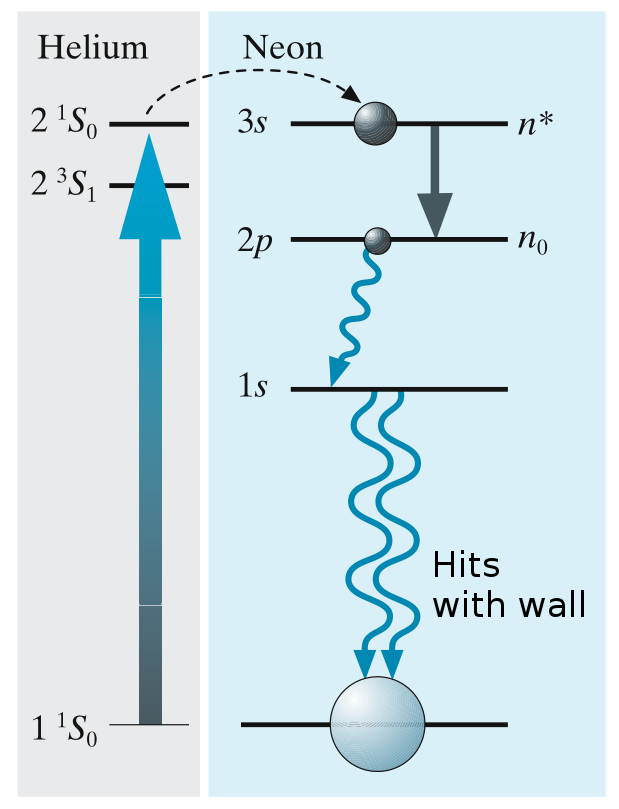
\includegraphics[width=8cm]{figures/helium-neon-laser}
        \label{fig:integral}
    \end{centering}
\end{SCfigure}

\begin{figure}
    \begin{centering}
    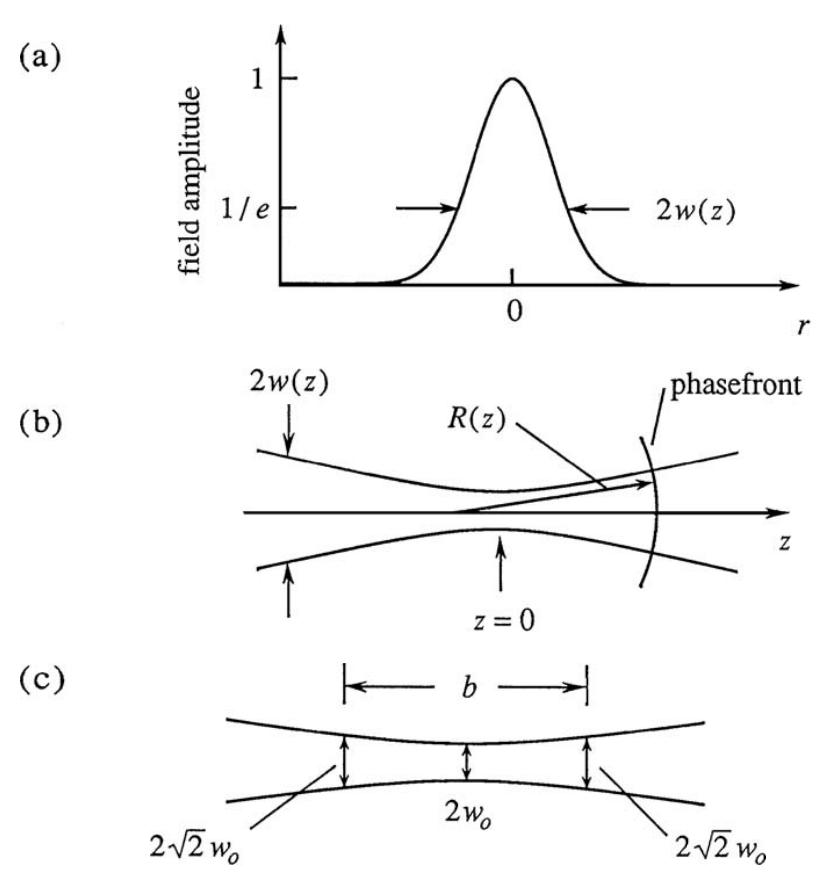
\includegraphics[width=13cm]{figures/gaussian}
    \caption{Different aspects of the gaussian nature of the laser beam~\cite{boyd2003nonlinear}.
        (a) Field amplitude distribution of a gaussian laser beam. (b) Variation of the beam
        radius $w$ and wavefront radius of curvature R with position $z$.
        (c) Relation between the beam waist radius and the confocal parameter $b$. }
    \end{centering}
\end{figure}
The beam waist radius $w_{0}$ can be calculated in terms of the Power $P$, which we can retrieve
by integrating:
\begin{equation}
    P = n \epsilon_0 c \pi w_0^2 |E_0|^2
\end{equation}
Unfortunatelly in our experimental setup it was neither possible to modificate the position of
the laser nor to adjust the setup in a way that we could have measured the specifications of 
the laser, so it is not possible for us to include dispersion or diffraction phenomena originating
from the gaussian nature of the beam into our considerations regarding to the analysis of the 
experiment. We added some notes in the chapter~\ref{sec:laser} ``
Further investigations regarding the laser''.


\clearpage
\newcommand{\figdirpockels}{analysis_pockels/figures/}

\section{Measurements for Pockels effect}
\subsection{Inspection without applied field}
\paragraph{Diffraction and Bifringence}
The inspection of the experimental setup revealed certain aspects
which we might need to include in our interpretation of the results
later. First we noticed minor diffraction phenomena already between
the exit of the Laser's Gaussian Beam and the beginning of the
Pockelcell, as well as bifringence phenomena which caused difficulties
in focusing the laser.  
\paragraph{Low frequency oscillations} Within the lasersignal 
we observed frequencies about $20 Hz$ with a intensity of $10mV/$diff.
We did not expect these frequencies at first; we will look into it
in the later progress of the experiment.
\subsection{Sawtooth signal}
We did now certain measurements for analyzing the behaviour of a 
certain degree of the analysator.

\begin{figure}
    \begin{subfigure}[b]{\picwidth}
        \includegraphics[width=\textwidth]{\figdirpockels 12sawtooth1}
        \caption{}
    \end{subfigure}\qquad
    \begin{subfigure}[b]{\picwidth}
        \includegraphics[width=\textwidth]{\figdirpockels 12sawtooth2}
        \caption{}
    \end{subfigure}
    \begin{subfigure}[b]{\picwidth}
        \includegraphics[width=\textwidth]{\figdirpockels 12sawtooth3}
        \caption{}
    \end{subfigure}
    \begin{subfigure}[b]{\picwidth}
        \includegraphics[width=\textwidth]{\figdirpockels 12sawtooth4}
        \caption{}
    \end{subfigure}
    \caption{These were the first measurements with the 
        oscillscope in order to calibrate the Analysator.
        The next measurements will show the result of the 
        final calibration. You can find the same configuration
        with different zoom from (b) to (d).}
    \label{fig:saw1}
\end{figure}
\flushleft
\begin{figure}
    \begin{subfigure}[b]{\picwidth}
        \includegraphics[width=\textwidth]{\figdirpockels 12sawtooth5}
        \caption{}
    \end{subfigure}\qquad
    \begin{subfigure}[b]{\picwidth}
        \includegraphics[width=\textwidth]{\figdirpockels 12sawtooth6}
        \caption{}
    \end{subfigure}
    \begin{subfigure}[b]{\picwidth}
        \includegraphics[width=\textwidth]{\figdirpockels 12sawtooth7}
        \caption{}
    \end{subfigure}
    \begin{subfigure}[b]{\picwidth}
        \includegraphics[width=\textwidth]{\figdirpockels 12sawtooth8}
        \caption{}
    \end{subfigure}
    \begin{subfigure}[b]{\picwidth}
        \includegraphics[width=\textwidth]{\figdirpockels 12sawtooth9}
        \caption{}
    \end{subfigure}
    \begin{subfigure}[b]{\picwidth}
        \includegraphics[width=\textwidth]{\figdirpockels 12sawtooth10}
        \caption{}
    \end{subfigure}

    \caption{These series of figures show the further 
        attempts to calibrate the analysator. As you can
        notice every figure shows a different degree of the 
        angle and hence the distribution of voltage changes. }
    \label{fig:saw2}
\end{figure}
\flushleft
\subsection{Sinus signal: Without direct current}
The Frequency generated was about $f=5.4$ Khz, but it was not stable
but oscillating within $0.1$ Khz. The manipulation of the trigger-
level increased the stability to a acceptable level. 
\subsection{Sinus signal: Applying Direct Current}
Now we will look at the inluence of different parameters on
the received signal, especially the effect of changing the
voltage. 
\paragraph{Important note:} After the measurements the
signalfrequency of the electrical field has gone up to 
$f=6.129$ khz! We noticed this without us to regulate this 
behavior. After the measurements we have changed this frequency in
order to the into account the change of frequency by adjusting.
We furthermore note that the change of frequency
does not seem to have a huge influence on the noisy regime except
that by reducing the frequency to $f=3.0$kHz we see the increase
of structure, meaning less noise and a clearly recognizable
sinusshape in the former noisy shape while the noisy regime
was shifted to other lower frequencies. We will look more refined
into this behavior in the next chapter.
\begin{figure}
    \begin{subfigure}[b]{\picwidth}
        \includegraphics[width=\textwidth]{\figdirpockels 22sinus01}
        \caption{}
    \end{subfigure}\qquad
    \begin{subfigure}[b]{\picwidth}
        \includegraphics[width=\textwidth]{\figdirpockels 22sinus02}
        \caption{}
    \end{subfigure}
    \begin{subfigure}[b]{\picwidth}
        \includegraphics[width=\textwidth]{\figdirpockels 22sinus03}
        \caption{}
    \end{subfigure}
    \begin{subfigure}[b]{\picwidth}
        \includegraphics[width=\textwidth]{\figdirpockels 22sinus04}
        \caption{}
    \end{subfigure}
    \begin{subfigure}[b]{\picwidth}
        \includegraphics[width=\textwidth]{\figdirpockels 22sinus05}
        \caption{}
    \end{subfigure}
    \begin{subfigure}[b]{\picwidth}
        \includegraphics[width=\textwidth]{\figdirpockels 22sinus06}
        \caption{}
    \end{subfigure}

    \caption{These series of figures show the impact of
        an applied sinussignal and a direct current with
        varying voltage. In general we do not recognize huge 
        qualitative differences amongst those, but we will look
        later with a more refined analysis to it.}
    \label{fig:sinus1}
\end{figure}
\flushleft
\begin{figure}
    \begin{subfigure}[b]{\picwidth}
        \includegraphics[width=\textwidth]{\figdirpockels 22sinus07}
        \caption{}
    \end{subfigure}\qquad
    \begin{subfigure}[b]{\picwidth}
        \includegraphics[width=\textwidth]{\figdirpockels 22sinus08}
        \caption{}
    \end{subfigure}
    \begin{subfigure}[b]{\picwidth}
        \includegraphics[width=\textwidth]{\figdirpockels 22sinus09}
        \caption{}
    \end{subfigure}
    \begin{subfigure}[b]{\picwidth}
        \includegraphics[width=\textwidth]{\figdirpockels 22sinus10}
        \caption{}
    \end{subfigure}
    \begin{subfigure}[b]{\picwidth}
        \includegraphics[width=\textwidth]{\figdirpockels 22sinus11}
        \caption{}
    \end{subfigure}
    \begin{subfigure}[b]{\picwidth}
        \includegraphics[width=\textwidth]{\figdirpockels 22sinus12}
        \caption{}
    \end{subfigure}

    \caption{Now we enter the noisy regime in which we can 
        observe the effect of the state of the analysator. 
        Here we are indulged to find the noisiest curve in 
        order to check the range in which the $U_{\lambda / 2}$
        might be to find. As you will notice from the figures we
        suspect it to be in the range from $144.4V$ to $148.0V$
        but also see the next series of figures.}
    \label{fig:sinus2}
\end{figure}
\subsection{Refined frequency analysis}
The figures in this section are accomplished with $U_{DC}=145.8 V$.
In this analysis we investigate the effect of the frequency
on the regime in which we get a rather noisy signal. 

After
adjusting to a relatively low frequency $f=2.0$ kHz we changed
the frequencyrange on the oscillscope from 
$[1 - 25]$kHz to $[35 - 2500]$ Hz in order to stabilize the signal.
Now since we have found the frequency with which we have a chance
to find the already mentioned frequency-doubling, we will
\begin{figure}
    \includegraphics[width=15cm]{\figdirpockels 23sinus02}
    \caption{At this level the regime of the voltage is shifted
        again, but in this case to a higher value. Unfortunatelly
        at this high frequency it is not possible to distinguish
        clearly between the different regimes because the signal
        is very noisy at all voltages (due to shackling 
            and wiggling).}
\end{figure}
\clearpage
\subsection{Reanalysis at the lower frequency}
At the frequency $f=1$kHz we repeat now the former analysis and are
able to search after the so called \textit{frequency doubling}.
The signal is much more stable compared to the higher frequencies 
with regards to the noise and we will see in the analysis that
it is even possible to interpolate the regime we are searching after.
Therefore we inspect the curves from $U=135$V up to $U=142$V.
\begin{figure}
    \begin{subfigure}[b]{\picwidth}
        \includegraphics[width=\textwidth]{\figdirpockels 24sinus01}
        \caption{}
    \end{subfigure}
    \begin{subfigure}[b]{\picwidth}
        \includegraphics[width=\textwidth]{\figdirpockels 24sinus02}
        \caption{}
    \end{subfigure}
    \begin{subfigure}[b]{\picwidth}
        \includegraphics[width=\textwidth]{\figdirpockels 24sinus03}
        \caption{}
    \end{subfigure}
    \begin{subfigure}[b]{\picwidth}
        \includegraphics[width=\textwidth]{\figdirpockels 24sinus04}
        \caption{}
    \end{subfigure}
    \caption{Refined search for the noisy regime.}
    \label{fig:sinus7}
\end{figure}

\begin{figure}
    \begin{subfigure}[b]{\picwidth}
        \includegraphics[width=\textwidth]{\figdirpockels 24sinus05}
        \caption{}
    \end{subfigure}\qquad
    \begin{subfigure}[b]{\picwidth}
        \includegraphics[width=\textwidth]{\figdirpockels 24sinus06}
        \caption{}
    \end{subfigure}
    \begin{subfigure}[b]{\picwidth}
        \includegraphics[width=\textwidth]{\figdirpockels 24sinus07}
        \caption{}
    \end{subfigure}
    \begin{subfigure}[b]{\picwidth}
        \includegraphics[width=\textwidth]{\figdirpockels 24sinus08}
        \caption{}
    \end{subfigure}
    \begin{subfigure}[b]{\picwidth}
        \includegraphics[width=\textwidth]{\figdirpockels 24sinus09}
        \caption{}
    \end{subfigure}
    \begin{subfigure}[b]{\picwidth}
        \includegraphics[width=\textwidth]{\figdirpockels 24sinus10}
        \caption{}
    \end{subfigure}
    \caption{Refined search for the noisy regime.}
    \label{fig:sinus8}
\end{figure}
\subsection{Further investigations regarding the laser}\label{sec:laser}
Now we removed everything except from the photodiode and noticed that
the laser exhibits the noise signal which we found in the beginning
(see figure~\ref{fig:laser_a}). After this we also removed the
laser and noticed that the light coming from the ceiling was 
measured by the diode (see figure~\ref{fig:laser_b}).
After we added the laser again, the polarizator and the analysator
(see figure~\ref{fig:laser_f} ).
We can see that the polarization 
state of the laser does not change the noise signal which we 
tracked down in this analysis. 
\begin{figure}
    \begin{subfigure}[b]{\picwidth}
        \includegraphics[width=\textwidth]{\figdirpockels 24sinus20}
        \caption{}
    \end{subfigure}
    \begin{subfigure}[b]{\picwidth}
        \includegraphics[width=\textwidth]{\figdirpockels 25_laser01}
        \caption{}
        \label{fig:laser_a}
    \end{subfigure}
    \begin{subfigure}[b]{\picwidth}
        \includegraphics[width=\textwidth]{\figdirpockels 25_no_laser01}
        \caption{}
        \label{fig:laser_b}
    \end{subfigure}
    \begin{subfigure}[b]{\picwidth}
        \includegraphics[width=\textwidth]{\figdirpockels 25_laser05}
        \caption{}
        \label{fig:laser_f}
    \end{subfigure}

    \caption{As mentioned in the beginning, an underlying
        frequency of about $f=23$Hz is very visible (a) since 
            we are nearly in the range of that frequency.
        From (b) to (d) we removed the Pockelcell and the applied current and observed
        the laser alone.
        (b) and (d) show the very low frequency which
        the laser inhibits as a nuisance where at (c) we changed the state of the analysator
        such that the intensity was minimal. We expect this signal coming from the electronic components
        the laser consists of. Figure (b) shows the frequency only originating from the room light.
        }
    \label{fig:laser}
\end{figure}
\clearpage


\section{Evaluation for Pockels effects}
\subsection{Fourier analysis of frequencies}
As described before \ref{sec:pdf}, we use Fourier analysis to determine 
the input voltage $U_\mathrm{DC}$ at which frequency doubling occurs. 
To illustrate the procedure, we show an example at $U_\mathrm{DC} = 137.0$ V.
The cut-off is taken at $t = 1.1$ ms and $t = 9.05$ ms, as shown in figure 
\ref{fig:cut_off_example}. The result of the FFT is then shown in figure 
\ref{fig:fft_example} for a larger range of frequencies and those of interest, 
namly $\nu < 2$ kHz. One clearly observes the two peaks close to 
0.5 kHz and 1.0 kHz, being of the same scale. This procedure is 
done with all datasets corresponding to the signals shown in 
the figures \ref{fig:sinus8}, which has shown the largest 
change regarding frequency doubling by eye. The result of the fourier 
analysis in the range from $0$ to $2$ kHz as well as the 
value of $|\mathrm{FFT}\left[U_\mathrm{out} \left(\nu\right)\right]|^2$ for 
$\nu_1 = 0.45$ kHz and $\nu_2 = 0.91$ kHz 
is shown in figure \ref{fft_all}.
One can clearly observe the drop in amplitude for $U_\mathrm{DC} = 139.0$ kHz. 
We will thus take this to be our measured value for $\Ula$.
\begin{figure}
\includegraphics[width=\pltw]{figures/cut_off_example.pdf}
\caption{
    Example for cut off points, for measured data at 
    $U_\mathrm{DC} = 137.0$ V. The minima of the input 
    signal $U_\mathrm{in}$, which is shown rescaled in this plos, 
    are found numerically in the ranges 
    $t \in (1.0, 1.5)$ ms and $t \in (8.5, 9.5)$ ms. 
    Further window functions are not applied. 
    By eye, the frequency doubling is seen already. 
    }
\label{fig:cut_off_example}
\end{figure}

\begin{figure}
\includegraphics[width=\pltw]{figures/fft_example.pdf}
\caption{
    Example for results of fourier analysis, for measured data at 
    $U_\mathrm{DC} = 137.0$ V.
    On the larger range, one observes strong peaks for low frequencies 
    and one relatively high peak at $\nu = 35.0$ kHz, which will not be 
    subject to further analysis. On the reduced range, the two peaks 
    due to the input signal and frequency doubling can be observed. 
    }
\label{fig:fourier_example}
\end{figure}

\begin{figure}
\includegraphics[width=0.9\textwidth]{figures/fft_all.pdf}
\caption{
    Taken the quantity
    $|\mathrm{FFT}\left[U_\mathrm{out} \left(\nu\right)\right]|^2$ 
    for all datasets yields a fairly confusing image, 
    which is, however, instructive as one observes the 
    frequency doubling for the different direct currents 
    $U_\mathrm{DC}$.
    In the right plot, the minimum for the lower frequency indicates 
    the maximal frequency doubling. We expected a maximum in the 
    double frequency, which clearly doesn't show. This 
    may be due to the small size of the dataset (in terms 
        of $t$ or the number of oscillations). 
    }
\label{fig:fft_all}
\end{figure}



\subsection{Calculation of the electro-optic coefficient}
Now we can use the former calculation to calculate the electro-optic coefficient.
\begin{equation}
    r_{41} = \frac{\lambda d}{4 l U_{\lambda / 2}} 
    \left(\frac{1}{2} \left(\frac{1}{\eps_\perp} + \frac{1}{\eps_\parallel}\right)\right)^{\frac{3}{2}}
    \label{eq:r_41_U}
\end{equation}
Now we use the following parameters (these were given before):
\begin{itemize}
\setlength\itemsep{0em}
\item[] $\lambda = (632.8\pm 0.1)$nm
\item[] $n_1     = 1.522\pm 0.001$
\item[] $n_3     = 1.477\pm 0.001$
\item[] $l       = ( 20\pm 0.1)$mm
\item[] $d       = (2.4\pm 0.1)$mm
\end{itemize}
Now we can calculate $r_{41}$ with respect to $U_{\lambda/2}$ with two different methods.
\subsubsection{Saw tooth method}
\label{ssub:Saw tooth method}

\subsubsection{DC current method}
\label{ssub:DC current method}
We estimated $U_{\lambda/2}    = (135  \pm 15)$.
% r !python analysis_pockels/r41_calc.py
Our result is the following: 
\begin{equation*}
r_{41} = \left (20.9 \pm 2.5 \right )  \mathrm{pm}
\end{equation*}

\clearpage

% Faraday
\section{Theory behind the Faraday effect}
The \textit{Faradayeffect} refers to a megneto-optical phenomenon which can be explained in terms
of circular birefringence. The effect causes a rotation of the polarization direction with regards
to a applied magnetic field and its direction. It was discovered by \textit{faraday} in 1845 and
can be seen as the first experiment showing the interplay between light and electromagnetism. 
As already mentioned in the first part we can use the Maxwell equations to describe the magnetic
and electric field such that we can understand how the dielectricity of the material gives rise
to the phenomenon. For the experimental setup for seeing the faradayeffect you insert a medium,
which does not have to be optically active, between two polarizators. If we now fix the direction
of the magnetic field to be parallel to the direction of the incoming light we observe the 
already mentioned rotation.   
\subsection{Magneto-optic rotation}
As it turns out the first approximation the rotation angle of the polarization is proportional
to the Depth of the material $l$ and the magnetic field $B$:
\begin{equation}
    \alpha = V l B
\end{equation}
Where we introduced the Verdet-constant $V$. In the following we will derive this formula in order
to understand the physical nature of this constant \cite{staatsexamen}.
Lets assume without loss of generality a plane wave solution to the maxwell equation
with propagation in $z$-direction with speed v, 
entering the medium at $z=$, being turned with the angle
$\alpha = \phi  z$:
\begin{align}
x &= F \cos{(\phi z)} \cos{\left ( \omega \left ( t - \frac{z}{v} \right )\right)} \\ 
y &= F \sin{(\phi z)} \cos{\left ( \omega \left ( t - \frac{z}{v} \right )\right)}
\end{align}
if we now apply $\cos(\beta) = (e^{i\beta} + e^{-i\beta})/2$ 
(analogous $\sin(\beta) = (e^{i\beta} - e^{-i\beta})/2i$ )
and rename $\tau := (t-\frac{z}{v})$:
\begin{align}
x &= \frac{F}{4} \left (e ^{i\phi z} + e ^{-i\phi z} \right )
\left (e ^{i\omega \tau} + e ^{-i\omega \tau} \right ) \\ 
&= \frac{F}{2} \left ( \cos{(\phi z + \omega \tau)} + \cos{(\omega \tau -  \phi z )} \right ) \\
\Rightarrow y &= \frac{F}{2} \left ( \sin{(\phi z + \omega \tau)} - \sin{(\omega \tau -  \phi z )} \right )
\end{align}
which in particular shows how the linear polarized wave consists of two circular, reverse polarized
waves with relatives speeds:
\begin{align}
\frac{\omega}{v_+} &= \frac{\omega}{v} - \phi \label{eq:v+}\\ 
\frac{\omega}{v_-} &= \frac{\omega}{v} + \phi \label{eq:v-}
\end{align}
Subtracting these two equations yields
\begin{equation}
2\phi = \omega \left (\frac{1}{v_-} - \frac{1}{v_+} \right)
\end{equation}
which we can insert into the definition of $\alpha$ and the refraction index $n = c/v$:
\begin{align}
\alpha = \phi l &= \frac{\omega l}{2} \left (\frac{1}{v_-} - \frac{1}{v_+} \right) \\ 
 &= \frac{\omega l}{2c} \left (n_- - n_+ \right)
\end{align}
From equation \eqref{eq:v+} and \eqref{eq:v-} we get (implying for small $\phi$ in the last step):
\begin{equation}
v_{+/-} = \frac{\omega}{\frac{\omega}{v} \mp \phi} = \frac{v}{1 \mp \frac{\phi v}{\omega}} 
= v \left ( 1 \pm \frac{\phi v}{\omega}+ \left (\frac{\phi v}{\omega} \right)^2
\pm \left (\frac{\phi v}{\omega} \right)^3 + \left (\frac{\phi v}{\omega} \right)^4+ \cdots \right)
\approx v \left  (1 \pm \frac{\phi v}{\omega} \right )
\end{equation}
Using the semiclassical Bohrmodel we can understand the behavior of the electrons in 
first approximation with the Larmorfrequency:
\begin{equation}
\omega_L = \frac{-e B}{2 m c}
\end{equation}
Since the dynamics of the electrons is fundamentally connected to the dispersion of the material,
we can use this frequency to connect the Rotation of the polarization with the dynamical behavior 
of the electrons of the medium. If we go into a coordinatesystem which is rotating with $\omega_L$,
the electrons have their original frequency (predicted by the Bohr model), hence the electromagnetic
wave is shifted by this frequency with regards to the original coordinate system. Thus we get:
\begin{equation}
\alpha = \frac{\omega l}{2c} \left (n_{\omega + \omega_L} - n_{\omega - \omega_L}\right )  
\end{equation}
The refraction index in dependence of the frequency is given by the dispersion relation, which is 
dependent on the medium. For small frequencies we can taylor: 
\begin{equation}
n(\omega + \omega_L) \approx n(\omega) \pm \omega_L \frac{\partial n}{\partial \omega}
\end{equation}
and now we can write in this in terms of $\omega \frac{n}{w} = -\lambda \frac{n}{\lambda}$:
\begin{equation}
\alpha = \frac{\omega_L l \lambda}{c} \frac{\partial n}{\partial \lambda} = 
\frac{e l B \lambda}{2m c^2} \frac{\partial n}{\partial \lambda} \quad \text{Formula of Bequerel}
\end{equation}

\subsection{Half shade polarimeter}

\subsection{Experimental setup}

\subsection{Method of measuring the rotation angle}

\subsection{Method of measuring angle between dirctions of polarization of half-shade polarimeter}

 
\clearpage
\section{Measurements for Faraday effect}
\subsection{Inspection of the experiment}
\subsubsection{Observations}
The very first measurement with $I=0.0A$ yields as expected a rotation of the polarization
with $\alpha = 0.6 \pm 0.2$. We will choose the reference state of half-shade Polarimeter 
to be clearly dark, since the precision is best in this case.



    \begin{table}[htdp]
        \begin{tabular}{|l||p{1.1cm}|p{1.1cm}|p{1.1cm}|p{1.1cm}|p{1.1cm}|p{1.1cm}|p{1.1cm}|p{1.1cm}|p{1.1cm}|p{1.1cm}|}
        \hline
            \multicolumn{11}{|c|}{\cellcolor[RGB]{206,250,201}$
            \mathbf{Measurement \quad 2.1}$} \\
\textbf{angle $\alpha$}& 0.60& 0.90& 1.60& 2.00& 2.50& 3.10& 3.40& 3.60& 4.40& 5.10 \\
\textbf{Current $I$}& 0.00& 0.20& 0.40& 0.60& 0.80& 1.00& 1.20& 1.40& 1.60& 1.80 \\

        \hline
        \end{tabular}
        \begin{tabular}{|l||p{1.1cm}|p{1.1cm}|p{1.1cm}|p{1.1cm}|p{1.1cm}|p{1.1cm}|p{1.1cm}|p{1.1cm}|p{1.1cm}|p{1.1cm}|}
        \hline\textbf{angle $\alpha$}& 5.70& 6.30& 6.70& 7.10& 7.90& 8.00& 8.40& 9.20& 9.50& 10.10 \\
\textbf{Current $I$}& 2.00& 2.20& 2.40& 2.60& 2.80& 3.00& 3.20& 3.40& 3.60& 3.80 \\

        \hline
        \end{tabular}
    \begin{tabular}{|l||p{1.1cm}|p{1.1cm}|p{1.1cm}|p{1.1cm}|p{1.1cm}|p{1.1cm}|}
    \hline\textbf{angle $\alpha$}& 10.70& 11.20& 11.70& 12.40& 12.80& 13.10 \\
\textbf{Current $I$}& 4.00& 4.20& 4.40& 4.60& 4.80& 4.94 \\

    \hline
    \end{tabular}
    \caption{}
    \label{Power05}
    \end{table}

    \begin{table}[htdp]
        \begin{tabular}{|l||p{1.1cm}|p{1.1cm}|p{1.1cm}|p{1.1cm}|p{1.1cm}|p{1.1cm}|p{1.1cm}|p{1.1cm}|p{1.1cm}|p{1.1cm}|}
        \hline
            \multicolumn{11}{|c|}{\cellcolor[RGB]{206,250,201}$
            \mathbf{Measurement \quad 2.2}$} \\
\textbf{angle $\alpha$}& 0.80& -0.40& -0.50& -1.10& -1.70& -1.90& -2.70& -3.20& -4.00& -4.20 \\
\textbf{Current $I$}& 0.00& -0.20& -0.40& -0.60& -0.80& -1.00& -1.20& -1.40& -1.60& -1.80 \\

        \hline
        \end{tabular}
        \begin{tabular}{|l||p{1.1cm}|p{1.1cm}|p{1.1cm}|p{1.1cm}|p{1.1cm}|p{1.1cm}|p{1.1cm}|p{1.1cm}|p{1.1cm}|p{1.1cm}|}
        \hline\textbf{angle $\alpha$}& -4.90& -5.50& -5.70& -6.20& -6.80& -7.10& -7.60& -8.70& -9.50& -10.00 \\
\textbf{Current $I$}& -2.00& -2.20& -2.40& -2.60& -2.80& -3.00& -3.20& -3.60& -3.80& -4.00 \\

        \hline
        \end{tabular}
    \begin{tabular}{|l||p{1.1cm}|p{1.1cm}|p{1.1cm}|p{1.1cm}|p{1.1cm}|}
    \hline\textbf{angle $\alpha$}& -10.40& -10.80& -11.40& -11.80& -12.10 \\
\textbf{Current $I$}& -4.20& -4.40& -4.60& -4.80& -4.90 \\

    \hline
    \end{tabular}
    \caption{}
    \label{Power05}
    \end{table}

    \begin{table}[htdp]
        \begin{tabular}{|l||p{1.1cm}|p{1.1cm}|p{1.1cm}|p{1.1cm}|p{1.1cm}|p{1.1cm}|p{1.1cm}|p{1.1cm}|p{1.1cm}|p{1.1cm}|}
        \hline
            \multicolumn{11}{|c|}{\cellcolor[RGB]{206,250,201}$
            \mathbf{Measurement \quad 2.3}$} \\
\textbf{angle $\alpha$}& 1.50& 2.20& 2.80& 3.10& 3.20& 3.60& 3.80& 3.90& 4.10& 4.20 \\
\textbf{Current $I$}& 0.40& 0.79& 0.94& 1.03& 1.11& 1.27& 1.33& 1.37& 1.42& 1.48 \\

        \hline
        \end{tabular}
        \begin{tabular}{|l||p{1.1cm}|p{1.1cm}|p{1.1cm}|p{1.1cm}|p{1.1cm}|p{1.1cm}|p{1.1cm}|p{1.1cm}|p{1.1cm}|p{1.1cm}|}
        \hline\textbf{angle $\alpha$}& 4.60& 5.70& 5.80& 6.10& 6.70& 7.10& 7.90& 8.20& 8.30& 8.50 \\
\textbf{Current $I$}& 1.64& 1.99& 2.07& 2.21& 2.44& 2.59& 2.90& 3.00& 3.06& 3.14 \\

        \hline
        \end{tabular}
    \begin{tabular}{|l||p{1.1cm}|p{1.1cm}|p{1.1cm}|p{1.1cm}|p{1.1cm}|p{1.1cm}|}
    \hline\textbf{angle $\alpha$}& 9.90& 10.30& 11.00& 11.60& 11.80& 12.40 \\
\textbf{Current $I$}& 3.69& 3.83& 4.07& 4.35& 4.40& 4.59 \\

    \hline
    \end{tabular}
    \caption{}
    \label{Power05}
    \end{table}

    \begin{table}[htdp]
        \begin{tabular}{|l||p{1.1cm}|p{1.1cm}|p{1.1cm}|p{1.1cm}|p{1.1cm}|p{1.1cm}|p{1.1cm}|p{1.1cm}|p{1.1cm}|p{1.1cm}|}
        \hline
            \multicolumn{11}{|c|}{\cellcolor[RGB]{206,250,201}$
            \mathbf{Measurement \quad 2.4}$} \\
\textbf{angle $\alpha$}& 0.50& 0.80& 1.40& 1.80& 2.30& 2.90& 3.60& 4.10& 4.30& 4.90 \\
\textbf{Current $I$}& 0.00& 0.20& 0.40& 0.60& 0.80& 1.00& 1.20& 1.40& 1.60& 1.80 \\

        \hline
        \end{tabular}
        \begin{tabular}{|l||p{1.1cm}|p{1.1cm}|p{1.1cm}|p{1.1cm}|p{1.1cm}|p{1.1cm}|p{1.1cm}|p{1.1cm}|p{1.1cm}|p{1.1cm}|}
        \hline\textbf{angle $\alpha$}& 5.50& 6.20& 6.50& 7.10& 7.60& 8.00& 8.70& 8.90& 9.50& 10.20 \\
\textbf{Current $I$}& 2.00& 2.20& 2.40& 2.60& 2.80& 3.00& 3.20& 3.40& 3.60& 3.80 \\

        \hline
        \end{tabular}
    \begin{tabular}{|l||p{1.1cm}|p{1.1cm}|p{1.1cm}|p{1.1cm}|p{1.1cm}|}
    \hline\textbf{angle $\alpha$}& 10.80& 11.30& 11.60& 12.10& 12.20 \\
\textbf{Current $I$}& 4.00& 4.20& 4.40& 4.60& 4.70 \\

    \hline
    \end{tabular}
    \caption{}
    \label{Power05}
    \end{table}

\clearpage
\section{Evaluation for Faraday effect}
Now we fitted the plots with a leastsquare linear polynomial. 
The reasoning behind is, that the given standard deviations 
seem to be estimated much to high - one would expect more fluctuation 
around the fitted polynome. This observation can be made more 
precise using the $\chi^2$-test. For a variable $y_i$ in a sample of 
size $N$ assumed to follow 
a gaussian disribution around its expectation value, which in case of 
an underlying functional relation to another variable $x_i$ is assumed 
to be $\lambda(x_i; \theta)$, where $\theta$ are the parameters of 
the fit, we can define the quantity
\begin{equation}
    \chi^2(\theta) = \sum_{i, j= 1}^N (y_i - \lambda(x_i; \theta))
        (V^{-1}) (y_j - \lambda(x_j; \theta)), 
\end{equation}
where $V^{-1}$ is the inverse of the covariance matrix $\mathrm{cov}(i,j)$. 
The least square fit is done by simply minimizing the quantity. If the 
variables do follow the suspected functional relation and are distributed 
with a variance $\sigma_i^2$, then $chi^2$ should follow the 
$chi^2$-distribution with expectation value $n_d$, where $n_d$ is 
the number of points minus the number of paramter $\theta$.
One can thus test the applied hypothesis by calculating $chi^2$ and 
dividing it by $n_d$, getting a numerical value for the 
\emph{godness-of-fit}.
\begin{figure}
    \begin{centering}
        \includegraphics[width=18cm]{figures/fig21}
\captionsetup{singlelinecheck=off} 
\caption[.]{
\begin{eqnarray}
    \mathrm{cov}(p_i, p_j) &=& 
    \begin{pmatrix}
        4.511\mathrm{e}-04 &-1.127\mathrm{e}-03 \\
        -1.127\mathrm{e}-03 &3.824\mathrm{e}-03 \\
    \end{pmatrix}
\\ \Rightarrow \qquad
    p_1 &=& 2.561 \pm 0.021 \cm\\
    p_2 &=& 0.45 \pm 0.06 \cm \\ 
    \chi ^2/(N-1) &=&  0.092
\end{eqnarray}
}

    \end{centering}
\end{figure}
\begin{figure}
    \begin{centering}
        \includegraphics[width=18cm]{figures/fig22}
\captionsetup{singlelinecheck=off} 
\caption[.]{
\begin{eqnarray}
    \mathrm{cov}(p_i, p_j) &=& 
    \begin{pmatrix}
        3.835\mathrm{e}-03 &9.572\mathrm{e}-03 \\
        9.572\mathrm{e}-03 &3.245\mathrm{e}-02 \\
    \end{pmatrix}
\\ \Rightarrow \qquad
    p_1 &=& 2.53 \pm 0.06 \cm\\
    p_2 &=& 0.41 \pm 0.18 \cm \\
    \chi ^2/(N-1) &=& 0.114
\end{eqnarray}
}


%\label{fig:fig22}
    \end{centering}
\end{figure}

\begin{figure}
    \begin{centering}
        \includegraphics[width=18cm]{figures/fig23}
\captionsetup{singlelinecheck=off} 
\caption[.]{
\begin{eqnarray}
    \mathrm{cov}(p_i, p_j) &=& 
    \begin{pmatrix}
        1.443\mathrm{e}-04 &-3.391\mathrm{e}-04 \\
        -3.391\mathrm{e}-04 &1.014\mathrm{e}-03 \\
    \end{pmatrix}
\\ \Rightarrow \qquad
    p_1 &=& 2.606 \pm 0.012 \cm\\
    p_2 &=& 0.349 \pm 0.032 \cm \\
    \chi ^2/(N-1) &=&  0.020
\end{eqnarray}
}
    \end{centering}
\end{figure}

\begin{figure}
    \begin{centering}
        \includegraphics[width=18cm]{figures/fig24}
\captionsetup{singlelinecheck=off} 
\caption[.]{
\begin{eqnarray}
    \mathrm{cov}(p_i, p_j) &=& 
    \begin{pmatrix}
        3.310\mathrm{e}-04 &-7.931\mathrm{e}-04 \\
        -7.931\mathrm{e}-04 &2.582\mathrm{e}-03 \\
    \end{pmatrix}
\\ \Rightarrow \qquad
    p_1 &=& 2.561 \pm 0.018 \cm\\
    p_2 &=& 0.38 \pm 0.05 \cm \\
    \chi ^2/(N-1) &=&  0.060
\end{eqnarray}
}
    \end{centering}
\end{figure}


\begin{figure}
    \begin{centering}
        \includegraphics[width=18cm]{figures/fig_all}
\captionsetup{singlelinecheck=off} 
\caption[.]{
\begin{eqnarray}
    \mathrm{cov}(p_i, p_j) &=& 
    \begin{pmatrix}
        1.116\mathrm{e}-04 &-2.694\mathrm{e}-04 \\
        -2.694\mathrm{e}-04 &8.667\mathrm{e}-04 \\
    \end{pmatrix}
\\ \Rightarrow \qquad
    p_1 &=& 2.573 \pm 0.011 \cm\\
    p_2 &=& 0.398 \pm 0.029 \cm \\ 
    \chi ^2/(N-1) &=& 0.064
\end{eqnarray}
}
    \end{centering}
\end{figure}




\clearpage
\section{Conclusion}
In the first part of the experiment, we basically obtained one 
central results: The approximated band gap energy $E_g$ for germanium 
and silicon. Our measured values lie at 
\begin{align}
    E_{g, \mathrm{Si}} &= (1.14 \pm 0.05) \,\mathrm{eV} \\
    E_{g, \mathrm{Ge}} &= (0.69 \pm 0.03) \,\mathrm{eV}
\end{align}
Both values cover the literature values within one standard deviation.
This accuracy was a rather surprising result to us, as we expected the 
applied method to be of a much lower certainty. 

The values measured in the Haynes \& Shockley experiment 
are displayed in the table~\ref{tab:conc_h_s} below:
\renewcommand{\arraystretch}{1.5}
\begin{table}[H]
    \centering
    \caption{
        Results of the Haynes \& Shockley experiment, variating the 
        acceleration voltage or the distance between creating the 
        cloud of free charge and measuring it. The errors correspond 
        to propagated errors of fitting not including systematical ones 
        and are thus underestimated. 
        }
	\begin{tabular}{|p{4cm}|p{3cm}|p{3cm}|p{3cm}|}
		\hline
		\rowcolor{tabcolor}
		Parameter           & $U = \text{const.}$   & $d = \text{const.}$   & Literature~\cite{staatsexamen} \\ 
        \hline
        mobility $\mu_n$    & $2640 \pm 130$        & $3000 \pm 120$        & $3900$     \\
        life time $\tau_n$  & $6.7 \pm 1.0$         & $1.6 \pm 0.5$         & $45 \pm 2$ \\
        diffusion const. $D_n$ & $140 \pm 20$      & $130 \pm 20$          & $101$     \\
		\hline
	\end{tabular}
    \label{tab:conc_h_s}
\end{table}
For both the electron mobility and diffusion constant we observe agreement in the 
order of magnitude between our results and the given literature values. The 
errors are underestimated due to not including systematical errors in the calculation. 
Other the shortcomings of the electronics (which we experienced in terms 
of loosing the signal), it is clear that the experiment does not allow the 
measurement of these constants in a perfect crystal. This is especially 
true for the life time, which is one order of magnitude smaller then the 
accepted value for germanium. 

Examination of the two semiconductors Si and CdTe gave an insight into the 
characteristics that allow for the usage as detectors for ionizing 
radiation. The central result is the superiority of heavier materials
(here represented by CdTe) over light ones (Si) when the registration of as 
many events as possible is key. The quantitative result, 
the ratio of absorption coefficients has been estimated to be
\begin{align}
    \mathrm{\frac{Abs_{Si}}{Abs_{CdTe}}}(59.5\, \mathrm{keV}) &= (3.51 \pm 0.07) \\
    \mathrm{\frac{Abs_{Si}}{Abs_{CdTe}}}(122.06\, \mathrm{keV}) &= (1.16 \pm 0.08)\\ 
    \mathrm{\frac{Abs_{Si}}{Abs_{CdTe}}}(136.47\, \mathrm{keV}) &= (1.9 \pm 0.6) \, ,
\end{align}
agreeing with the literature values in order of magnitude. The errors 
are those obtained by numerical calculation and do not include 
systematical errors, such as impurities or errors induced by the electronics. 
With one setup and the two possible semiconductors as detectors, one 
would thus need to measure 30 to 60 times as long with the Si semiconductor 
to obtain the same number of counts and thus the same statistical error. 
As a second, somewhat less striking result, we calculated the 
relative energy resolution (RER). The main result here is the increasing 
resolution with increasing energy: The resolution at 122 keV Co peak is 
twice the one at the 59.5 keV Am peak for both semiconductors.  

All three experiments resulted in a good introduction into semiconductor physics. 
Especially the Haynes and Shockley experiment, notwithstanding the disagreement in 
numerical results, gave a nice insight into models of the reality in semiconductors. 


\cleardoublepage
\phantomsection
\addcontentsline{toc}{section}{Bibliography und List of figures}
\bibliographystyle{plain}
\bibliography{report}
%\listoffigures
\clearpage
\section{Appendix}
\subsection{Records Pockels effect}
\includegraphics[width=0.9\linewidth]{record/pockels1}
\newpage
\includegraphics[width=1.0\linewidth]{record/pockels2}
\newpage
\includegraphics[width=1.0\linewidth]{record/pockels3}
\newpage
\includegraphics[width=1.0\linewidth]{record/pockels4}
\newpage
\includegraphics[width=1.0\linewidth]{record/pockels5}
\newpage
\includegraphics[width=1.0\linewidth]{record/pockels6}
\newpage
\includegraphics[width=1.0\linewidth]{record/pockels7}
\newpage
\includegraphics[width=1.0\linewidth]{record/pockels9}
\newpage
\includegraphics[width=1.0\linewidth]{record/pockels9}
\newpage
\includegraphics[width=1.0\linewidth]{record/pockels10}
\newpage
\subsection{Records Faraday effect}
\includegraphics[width=0.9\linewidth]{record/faraday1}
\newpage
\includegraphics[width=1.0\linewidth]{record/faraday2}

\end{document}
